%! Unidad 13 — Termodinámica: sistemas, variables y procesos termodinámicos, trabajo y calor, criterio de signos, principio
%! cero y temperatura, propagación del calor, calor específico, calorimetría, cambios de estado, dilatación, trabajo de un gas y
%! diagramas p-V, energía interna y primer principio, entropía, segundo principio y máquinas térmicas (teoría, ejemplos
%! resueltos, ejercicios por apartados, lectura, prácticas y situación de aprendizaje)
%! Fuente: Fuentes/Fisica/Unidad 13 (capturas 452 —portada, mitad derecha— a 463 + solucionario).
%! Texto reescrito; datos de los ejercicios cambiados y recalculados; 1 cal = 4,18 J; R = 8,31 J/(mol·K); 1 atm = 101 325 Pa.
%! Figuras en images/UD13/: nuevas en html/ (principio_cero, escalas_temperatura, mecanismos_calor, cambios_estado,
%!   expansion_embolo, practica_nube), copiadas (PDF + SVG) de 4ESO/images/UD12 (particulas_temperatura, equilibrio_termico,
%!   joule, dilatacion, bimetal, balance_calorimetro, maquina_termica, motor_cuatro_tiempos, practica_calor_especifico) y de
%!   2BachQuimica/FigurasSVG/UD4_Termodinamica (sistemas = UD4_01, energia_interna = UD4_05, criterio_signos = UD4_06).
%!   Gráficas con pgfplots (curva de calentamiento del agua, diagramas p-V).

\section*{Para empezar: subir con aire caliente}
\addcontentsline{toc}{section}{Para empezar: subir con aire caliente}

Al amanecer, sobre los templos de Bagan (Birmania) o sobre los campos de Capadocia (Turquía), decenas de \textbf{globos
aerostáticos} se elevan en silencio. Su funcionamiento es sencillo: un quemador de propano calienta el aire del interior de la
vela; el aire caliente se dilata, se vuelve menos denso que el aire frío que lo rodea y el globo sube. Para bajar basta con dejar
que el aire se enfríe. ¿Qué tiene que ver el calor con el movimiento? ¿Se puede convertir todo el calor del quemador en trabajo
útil?

La \textbf{termodinámica} estudia los intercambios de energía en forma de \textbf{calor} y de \textbf{trabajo}. Está presente en la
física y en la química: en los motores de los coches, en los frigoríficos y las bombas de calor, en las centrales eléctricas, en
las corrientes oceánicas y en fenómenos meteorológicos como las DANA, en las reacciones químicas e incluso en nuestro propio
organismo, que intercambia continuamente materia y energía con el entorno. En esta unidad estudiaremos sus conceptos básicos y sus
tres principios: el \textbf{principio cero} (temperatura y equilibrio térmico), el \textbf{primero} (la conservación de la energía)
y el \textbf{segundo} (la entropía y el sentido de los procesos).

%========================================================================================
\section{Recuerda de la ESO}\label{sec:ud13-eso}
%========================================================================================

\paragraph{Volumen de un cilindro.} Es el área de la base por la altura: \(V = S\,h = \pi\,r^2\,h\). Lo usaremos para el gas
encerrado en un cilindro con un émbolo.

\paragraph{Magnitudes extensivas e intensivas.} Una magnitud es \textbf{extensiva} si su valor depende de la cantidad de materia
(masa, volumen, energía) e \textbf{intensiva} si no depende de ella (temperatura, presión, densidad). Un vaso de agua y una jarra de
agua a la misma temperatura tienen distinto volumen, pero la misma temperatura y la misma densidad.

\paragraph{Teoría cinético-molecular.} La materia está formada por partículas en continuo movimiento desordenado. La
\textbf{temperatura} de un cuerpo es una medida de la \textbf{energía cinética media} de sus partículas.

\paragraph{Presión.} Es la fuerza por unidad de superficie, \(p = F/S\). Su unidad en el SI es el \textbf{pascal} (\(\qty{1}{\pascal}
= \qty{1}{\newton\per\m\squared}\)). También se usan \(\qty{1}{\bar} = \qty{e5}{\pascal}\) y \(\qty{1}{\atm} = \qty{101325}{\pascal} =
\qty{760}{\mmHg}\).

\paragraph{Calor y calor específico.} El \textbf{calor} es energía en tránsito entre dos cuerpos a distinta temperatura; pasa del
más caliente al más frío hasta que se alcanza el \textbf{equilibrio térmico}. Cada sustancia necesita una cantidad distinta de
energía para calentarse: es su \textbf{calor específico}. Para que \qty{1}{\g} de agua suba \qty{1}{\degreeCelsius} hace falta
\qty{1}{\calorie}; para \qty{1}{\g} de hierro basta con \qty{0.11}{\calorie}.

\paragraph{Trabajo.} El trabajo de una fuerza constante es \(W = \vec F \cdot \Delta\vec r = F\,\Delta r\cos\alpha\) y se mide en
julios. Si empujamos el émbolo de una jeringa tapada, hacemos trabajo sobre el gas y le comunicamos energía.

\begin{exercise}
    Un cilindro tiene un radio interior de \qty{4}{\cm} y una altura de \qty{12}{\cm}. a) ¿Qué volumen de gas cabe dentro, en litros?
    b) ¿Qué presión ejerce una fuerza de \qty{50}{\newton} sobre un émbolo que cierra el cilindro?
    \begin{solu}
        a) \(V = \pi \cdot \num{0.04}^2 \cdot \num{0.12} = \qty{6.03e-4}{\m\cubed} = \textcolor{red}{\qty{0.603}{\litre}}\).
        b) \(p = \dfrac{F}{S} = \dfrac{50}{\pi \cdot \num{0.04}^2} = \textcolor{red}{\qty{9.95e3}{\pascal}}\).
    \end{solu}
\end{exercise}

%========================================================================================
\section{Introducción a la termodinámica}\label{sec:ud13-introduccion}
%========================================================================================

El dominio del fuego fue un punto de inflexión para la humanidad: permitió cocinar, calentarse y transformar materiales. Pero la
ciencia del calor no nació hasta el siglo \textsc{xix}, cuando la \textbf{máquina de vapor} obligó a entender cómo convertir calor
en movimiento. En 1824, el ingeniero francés \textbf{Sadi Carnot} estudió el rendimiento de estas máquinas y sentó las bases de la
termodinámica. El nombre procede del griego \textit{thermos} (calor) y \textit{dynamis} (fuerza): reúne la \textbf{termología}, que
estudiaba los fenómenos térmicos, y la \textbf{mecánica}, que estudiaba el movimiento, las fuerzas y el trabajo.

\begin{definition}[Termodinámica]
    Es la parte de la física que estudia los intercambios de energía, en forma de calor y de trabajo, entre un sistema y su
    entorno, y las transformaciones de una forma de energía en otra.
\end{definition}

La termodinámica estudia sistemas \textbf{macroscópicos}, formados por un número enorme de partículas, y se ocupa de sus estados de
\textbf{equilibrio}. Sus principios no se demuestran: son generalizaciones de la \textbf{experiencia} que nunca se han visto
contradichas. La parte de la termodinámica que estudia los intercambios de energía en las reacciones químicas se llama
\textbf{termoquímica} (ya la vimos en la sección~\ref{sec:ud6-energia}).

\subsection{Sistemas termodinámicos}

\begin{definition}[Sistema termodinámico]
    Es la porción del universo que queremos estudiar, separada del resto por una \textbf{pared} o frontera, real o imaginaria. Lo
    que queda fuera y puede intercambiar energía o materia con él es el \textbf{entorno}. Sistema y entorno forman el
    \textbf{universo}.
\end{definition}

Según lo que pueden intercambiar con el entorno, los sistemas son (figura~\ref{fig:ud13-sistemas}):
\begin{itemize}
    \item \textbf{Abiertos}: intercambian materia y energía. Por ejemplo, una cazuela destapada al fuego, una sauna (hay que aportar
    agua y calor) o un ser vivo.
    \item \textbf{Cerrados}: intercambian energía, pero no materia. Un termómetro clínico: su mercurio o su alcohol no salen, pero
    recibe calor del cuerpo.
    \item \textbf{Aislados}: no intercambian ni materia ni energía. Un termo de buena calidad bien cerrado se acerca a este modelo;
    en sentido estricto, el único sistema perfectamente aislado es el universo.
\end{itemize}

\begin{figure}[H]
    \centering
    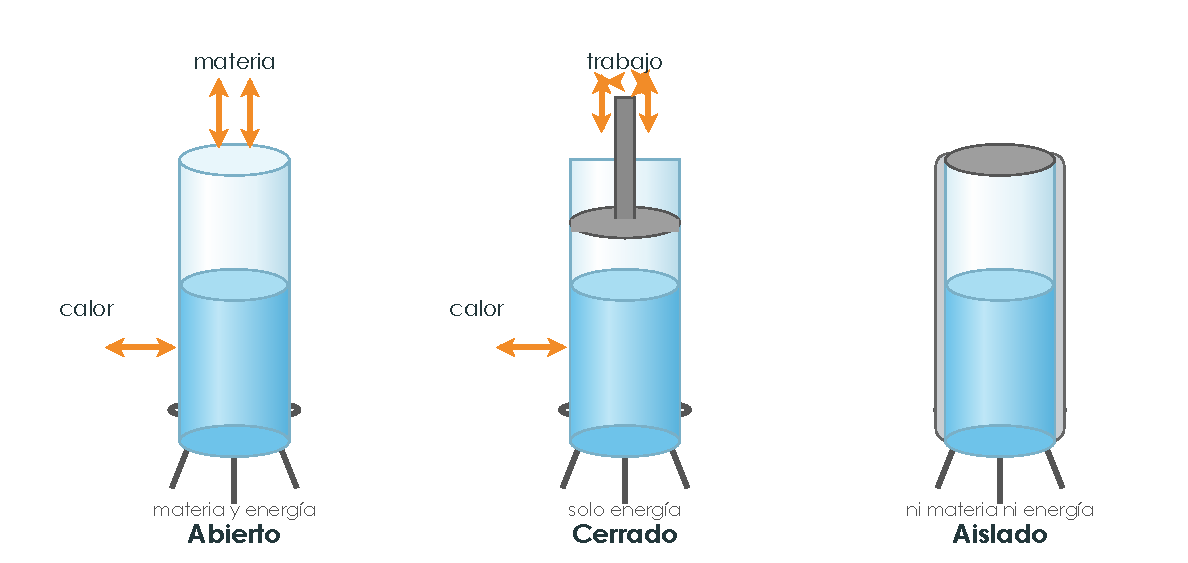
\includegraphics[width=0.7\textwidth]{images/UD13/sistemas}
    \caption{Sistemas abierto, cerrado y aislado.}
    \label{fig:ud13-sistemas}
\end{figure}

Las paredes del sistema determinan qué intercambios son posibles: las \textbf{rígidas} mantienen el volumen constante; las
\textbf{móviles} (como un émbolo) permiten que cambie el volumen e intercambiar trabajo; las \textbf{diatérmanas} dejan pasar el
calor, y las \textbf{adiabáticas} son aislantes térmicos ideales.

\subsection{Variables termodinámicas}

El \textbf{estado} de un sistema queda determinado por los valores de unas magnitudes macroscópicas medibles, las
\textbf{variables termodinámicas}: presión, volumen, temperatura, masa\dots{} Se pueden clasificar de dos formas
(tabla~\ref{tab:ud13-variables}).

\begin{table}[H]
    \centering
    \caption{Clasificación de las variables termodinámicas}
    \vspace{-5pt}
    \begin{tabular}{@{}lL{11cm}@{}}
        \toprule
        \textbf{Tipo} & \textbf{Características y ejemplos} \\
        \midrule
        Extensivas & Dependen de la cantidad de materia: masa \(m\), volumen \(V\), energía interna \(U\). \\[3pt]
        Intensivas & No dependen de la cantidad de materia; tienen un valor en cada punto: presión \(p\), temperatura \(T\),
        densidad \(\rho\). \\[3pt]
        \makecell[l]{Funciones \\ de estado} & Su variación depende solo de los estados inicial y final, no del camino seguido ni del
        tiempo empleado: \(p\), \(V\), \(T\), \(U\). \\[3pt]
        \makecell[l]{Variables de \\ transferencia} & Dependen del proceso seguido para ir de un estado a otro: calor \(Q\) y
        trabajo \(W\). \\
        \bottomrule
    \end{tabular}
    \label{tab:ud13-variables}
\end{table}

Una \textbf{ecuación de estado} relaciona entre sí varias funciones de estado. La más conocida es la de los gases ideales,
\(p\,V = n\,R\,T\), con \(R = \qty{8.31}{\joule\per\mol\per\kelvin} = \qty{0.082}{\atm\litre\per\mol\per\kelvin}\).

\begin{definition}[Proceso termodinámico]
    Es la evolución de un sistema desde un estado inicial \((p_0, V_0, T_0)\) hasta un estado final \((p_f, V_f, T_f)\).
\end{definition}

\begin{exercise}
    Clasifica estos sistemas en abiertos, cerrados o aislados: a) una lata de refresco cerrada; b) un termo de café bien tapado;
    c) una persona; d) una cafetera al fuego; e) un globo de helio atado; f) una planta; g) una nevera portátil cerrada; h) el
    planeta Tierra; i) una bolsa de palomitas en el microondas antes de abrirse.
    \begin{solu}
        \textcolor{red}{Abiertos}: c, d, f. \textcolor{red}{Cerrados}: a, e, h (intercambia energía con el Sol y el espacio, pero
        apenas materia), i. \textcolor{red}{Aislados} (aproximadamente): b, g.
    \end{solu}
\end{exercise}

\begin{exercise}
    Clasifica en extensivas o intensivas: masa, densidad, volumen, temperatura, energía interna, presión, calor específico y
    capacidad calorífica. ¿Se pueden incluir el calor y el trabajo en esta clasificación?
    \begin{solu}
        \textcolor{red}{Extensivas}: masa, volumen, energía interna y capacidad calorífica. \textcolor{red}{Intensivas}: densidad,
        temperatura, presión y calor específico. El calor y el trabajo \textcolor{red}{no}: no son propiedades del estado del
        sistema, sino energía que se transfiere durante un proceso.
    \end{solu}
\end{exercise}

\subsection{Trabajo y calor}

Decimos «¡qué calor hace!» o «este café tiene mucho calor», pero en física es incorrecto: los sistemas \textbf{no tienen} calor ni
trabajo. Calor y trabajo son \textbf{energía en tránsito}, las dos formas en que un sistema puede intercambiar energía con su
entorno:

\begin{itemize}
    \item \textbf{Calor} (\(Q\)): energía transferida debido a una \textbf{diferencia de temperatura} entre el sistema y el entorno.
    \item \textbf{Trabajo} (\(W\)): energía transferida mediante \textbf{fuerzas que producen desplazamientos}, por ejemplo al
    comprimir un gas o al agitar un líquido con unas paletas.
\end{itemize}

Ambos se miden en julios. Para el calor se usa también la \textbf{caloría}.

A mediados del siglo \textsc{xix}, \textbf{James Prescott Joule} demostró que el calor es una forma de energía y no una sustancia (el
«calórico» que se suponía entonces). En su aparato (figura~\ref{fig:ud13-joule}), unas pesas al caer hacen girar unas paletas dentro
del agua; el rozamiento de las paletas con el agua aumenta su temperatura. Midiendo la energía potencial perdida por las pesas y
el aumento de temperatura del agua, Joule obtuvo el \textbf{equivalente mecánico del calor}.

\begin{figure}[H]
    \centering
    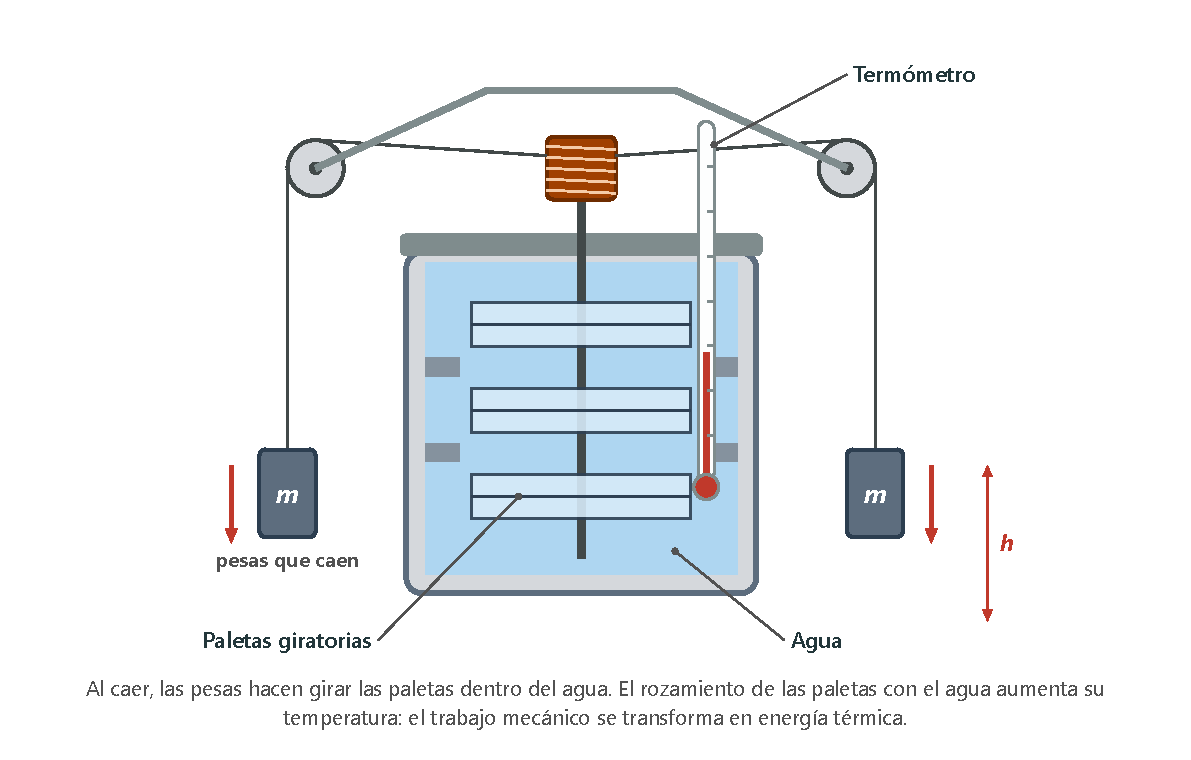
\includegraphics[width=0.65\textwidth]{images/UD13/joule}
    \caption{Experiencia de Joule: el trabajo de las pesas se convierte en energía térmica del agua.}
    \label{fig:ud13-joule}
\end{figure}

\begin{definition}[Caloría]
    Es la energía necesaria para elevar \qty{1}{\degreeCelsius} la temperatura de \qty{1}{\g} de agua a la presión de \qty{1}{\atm}.
    \[ \qty{1}{\calorie} = \qty{4.18}{\joule} \qquad \qty{1}{\joule} = \qty{0.24}{\calorie} \]
\end{definition}

\subsection{Criterio de signos}

Para indicar el sentido de los intercambios de energía, seguiremos el criterio de la \textbf{IUPAC} (llamado a veces «egoísta»,
porque se fija en lo que gana el sistema): \textbf{la energía que entra en el sistema es positiva y la que sale es negativa}
(figura~\ref{fig:ud13-signos}).

\begin{itemize}
    \item \(Q > 0\): el sistema absorbe calor. \(Q < 0\): el sistema cede calor.
    \item \(W > 0\): el entorno realiza trabajo sobre el sistema (compresión). \(W < 0\): el sistema realiza trabajo sobre el
    entorno (expansión).
\end{itemize}

\begin{figure}[H]
    \centering
    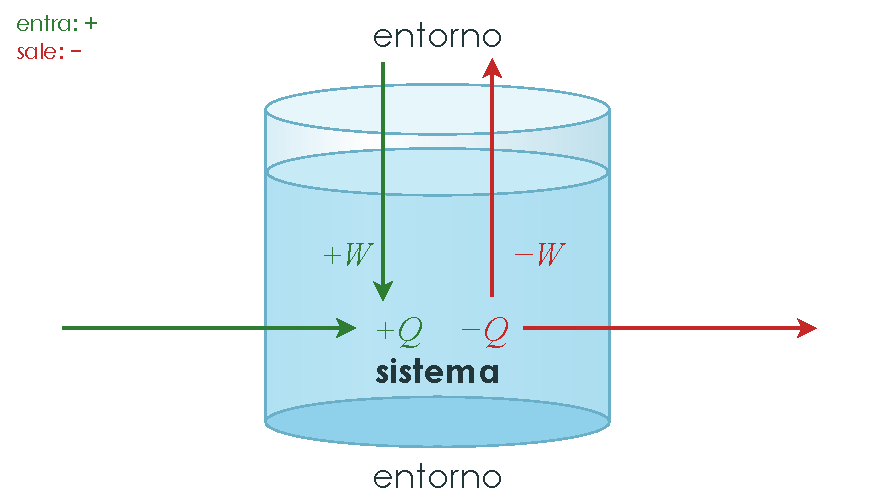
\includegraphics[width=0.45\textwidth]{images/UD13/criterio_signos}
    \caption{Criterio de signos de la IUPAC: lo que entra en el sistema es positivo.}
    \label{fig:ud13-signos}
\end{figure}

\begin{remark}
    En algunos textos de física e ingeniería se usa el criterio contrario para el trabajo (positivo el que hace el sistema), y el
    primer principio se escribe \(\Delta U = Q - W\). Las dos formas son equivalentes si se aplica cada una con su criterio.
\end{remark}

\subsection{Tipos de procesos termodinámicos}

Según si el sistema y el entorno pueden volver o no a su estado inicial, los procesos son:
\begin{itemize}
    \item \textbf{Irreversibles}: transcurren en un solo sentido; no se puede volver atrás sin dejar cambios en el entorno. Todos los
    procesos reales lo son en mayor o menor medida: una combustión, la mezcla de café y leche o el frenado de un coche.
    \item \textbf{Reversibles}: son una idealización; el sistema pasa por una sucesión de estados de equilibrio y se puede invertir
    con un cambio infinitesimal de las condiciones. Algunas reacciones químicas son reversibles, como la síntesis del amoniaco,
    \ch{N2 + 3 H2 <=> 2 NH3}.
\end{itemize}

Según la magnitud que permanece \textbf{constante} (tabla~\ref{tab:ud13-procesos}):

\begin{table}[H]
    \centering
    \caption{Procesos termodinámicos según la magnitud que se mantiene constante}
    \vspace{-5pt}
    \begin{tabular}{@{}llL{8.6cm}@{}}
        \toprule
        \textbf{Proceso} & \textbf{Constante} & \textbf{Ejemplo} \\
        \midrule
        Isobárico & presión, \(p\) & Reacciones en recipientes abiertos (a la presión atmosférica). \\[3pt]
        Isocórico & volumen, \(V\) & Cocinar en una olla exprés cerrada. \\[3pt]
        Isotérmico & temperatura, \(T\) & Fusión de un cubito de hielo: la temperatura se mantiene a \qty{0}{\degreeCelsius}
        hasta que se funde todo. \\[3pt]
        Adiabático & no hay calor, \(Q = 0\) & El gas que sale de un aerosol y se enfría; una compresión muy rápida. \\
        \bottomrule
    \end{tabular}
    \label{tab:ud13-procesos}
\end{table}

\subsection{Equilibrio termodinámico}

Un sistema está en \textbf{equilibrio termodinámico} cuando sus variables (presión, temperatura, composición\dots) no cambian con el
tiempo mientras nada lo perturbe desde el exterior. Si le aportamos calor o trabajo, rompemos ese equilibrio y el sistema evoluciona
hasta alcanzar un nuevo estado de equilibrio.

\begin{example}
    \textbf{¿Qué tipo de proceso es?} Clasifica estos procesos: a) cocer garbanzos en una olla exprés cerrada; b) se pincha una
    rueda y el aire sale de golpe; c) hervir agua en un cazo destapado; d) un cubito de hielo se funde en un vaso de agua con hielo.

    \textbf{Solución.} a) \textbf{Isocórico}: el volumen de la olla no cambia. b) \textbf{Adiabático}: el aire sale tan deprisa que
    no le da tiempo a intercambiar calor (por eso el aire que sale está frío). c) \textbf{Isobárico}: el cazo está abierto a la
    presión atmosférica; además, mientras hierve, la temperatura no cambia. d) \textbf{Isotérmico}: la mezcla de agua y hielo se
    mantiene a \qty{0}{\degreeCelsius}.
\end{example}

\begin{exercise}
    Escribe dos ejemplos de procesos reversibles y dos de procesos irreversibles de la vida cotidiana.
    \begin{solu}
        \textcolor{red}{Respuesta abierta}. Casi reversibles: fundir y volver a congelar un cubito; comprimir muy despacio el aire
        de una jeringa y dejarlo expandirse. Irreversibles: quemar un papel, romper un vaso, disolver azúcar en el café.
    \end{solu}
\end{exercise}

\begin{exercise}
    Explica con tus palabras el criterio de signos para el calor y el trabajo. Un gas encerrado en un cilindro recibe
    \qty{300}{\joule} de calor y empuja el émbolo realizando un trabajo de \qty{120}{\joule}. ¿Qué signos tienen \(Q\) y \(W\)?
    \begin{solu}
        Lo que entra en el sistema es positivo y lo que sale, negativo. \(Q = \textcolor{red}{\qty{+300}{\joule}}\) (entra calor);
        \(W = \textcolor{red}{\qty{-120}{\joule}}\) (el gas hace trabajo sobre el entorno y pierde energía).
    \end{solu}
\end{exercise}

\begin{exercise}
    ¿Es correcto decir que «la sopa tiene mucho calor»? ¿Cómo debería decirse?
    \begin{solu}
        \textcolor{red}{No}: los cuerpos no tienen calor, el calor es energía en tránsito. Debería decirse que la sopa
        \textcolor{red}{está a una temperatura alta} (o que tiene mucha energía interna) y que \textcolor{red}{puede ceder calor}
        a la boca.
    \end{solu}
\end{exercise}

%========================================================================================
\section{El principio cero de la termodinámica}\label{sec:ud13-principio-cero}
%========================================================================================

\subsection{Temperatura}

Calor y temperatura están relacionados, pero no son lo mismo: un cuerpo \textbf{tiene} una temperatura, pero no contiene calor.

\begin{definition}[Temperatura]
    Es la magnitud que mide la \textbf{energía cinética media} de las partículas de un sistema. Si aportamos energía a un sistema,
    sus partículas se mueven más deprisa en promedio y su temperatura aumenta (figura~\ref{fig:ud13-particulas}).
\end{definition}

\begin{figure}[H]
    \centering
    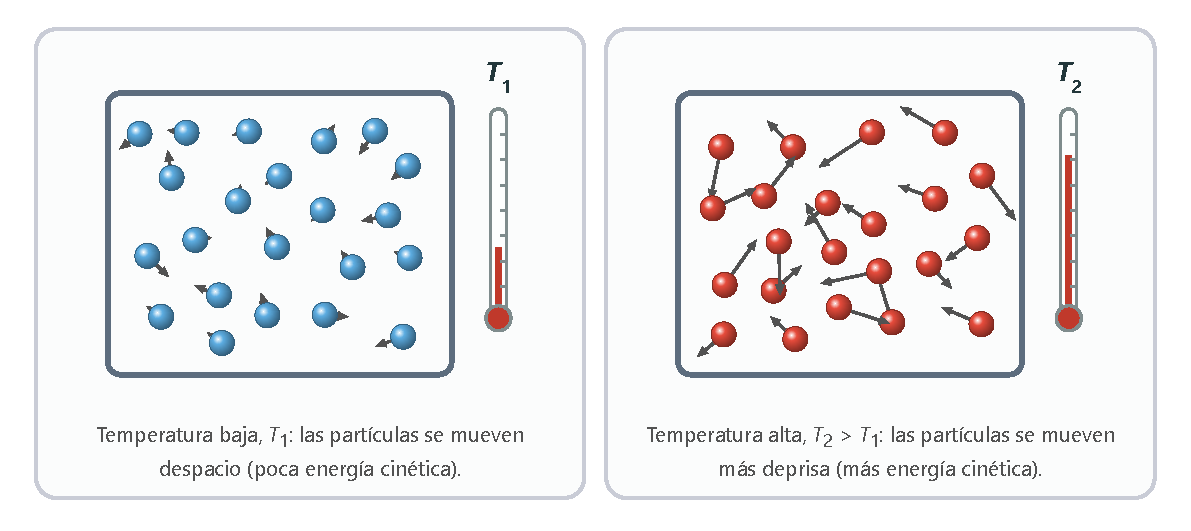
\includegraphics[width=0.8\textwidth]{images/UD13/particulas_temperatura}
    \caption{A mayor temperatura, mayor energía cinética media de las partículas.}
    \label{fig:ud13-particulas}
\end{figure}

Para medir la temperatura usamos \textbf{termómetros}, basados en \textbf{propiedades termométricas}, magnitudes que cambian con la
temperatura: la longitud de una columna de líquido, la presión de un gas a volumen constante, la resistencia eléctrica de un metal
o la radiación infrarroja que emite un cuerpo. La unidad de temperatura en el SI es el \textbf{kelvin} (K), aunque en la vida
diaria usamos el grado Celsius (figura~\ref{fig:ud13-escalas}):
\begin{itemize}
    \item \textbf{Escala Celsius}: asigna \qty{0}{\degreeCelsius} a la fusión del hielo y \qty{100}{\degreeCelsius} a la ebullición
    del agua a \qty{1}{\atm}, y divide el intervalo en 100 partes.
    \item \textbf{Escala Kelvin} o absoluta: su cero es el \textbf{cero absoluto}, la temperatura más baja posible, en la que la
    agitación de las partículas sería mínima; equivale a \qty{-273.15}{\degreeCelsius}. No tiene valores negativos.
\end{itemize}
\[ T\,(\unit{\kelvin}) = t\,(\unit{\degreeCelsius}) + \num{273.15} \]
Como el tamaño del grado es el mismo en las dos escalas, una \textbf{variación} de temperatura vale lo mismo en kelvin que en grados
Celsius: \(\Delta T\,(\unit{\kelvin}) = \Delta t\,(\unit{\degreeCelsius})\). En los cálculos se suele redondear a 273.

\begin{figure}[H]
    \centering
    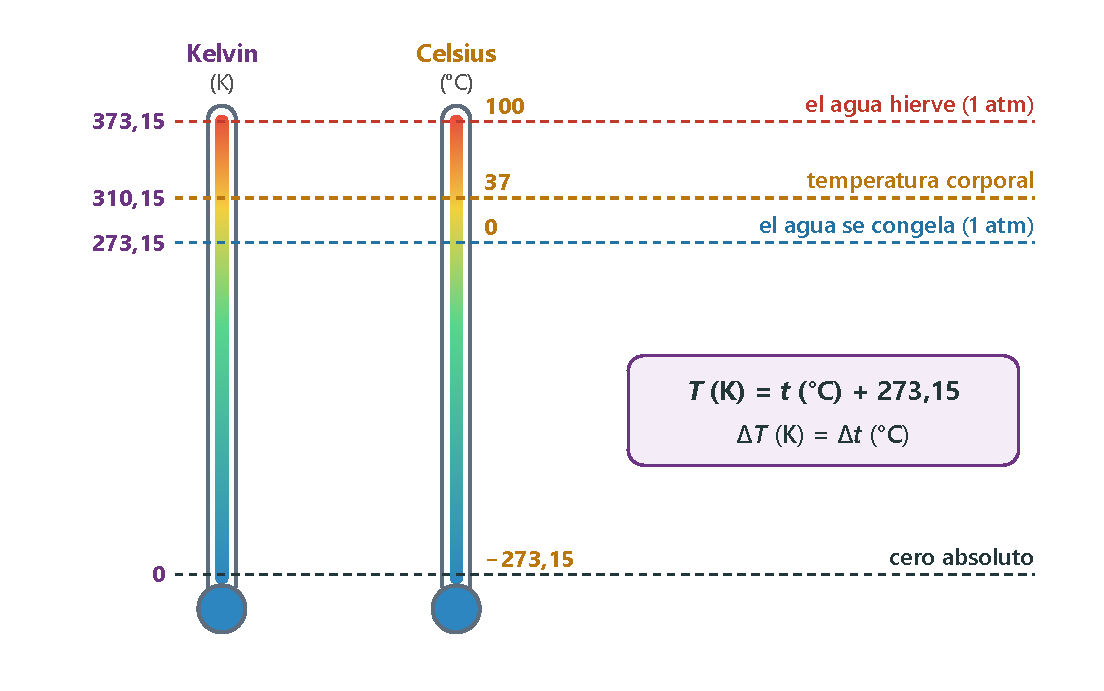
\includegraphics[width=0.7\textwidth]{images/UD13/escalas_temperatura}
    \caption{Relación entre las escalas Kelvin y Celsius.}
    \label{fig:ud13-escalas}
\end{figure}

\begin{example}
    \textbf{Cambios de escala.} a) Expresa en kelvin la temperatura de una persona con fiebre, \qty{38.5}{\degreeCelsius}.
    b) El nitrógeno líquido hierve a \qty{77}{\kelvin}: ¿a cuántos grados Celsius? c) Un día de verano la temperatura pasa de
    \qty{20}{\degreeCelsius} a \qty{38}{\degreeCelsius}; ¿cuánto vale la variación en kelvin?

    \textbf{Solución.} a) \(T = \num{38.5} + \num{273.15} = \qty{311.65}{\kelvin}\). b) \(t = 77 - \num{273.15} =
    \qty{-196.15}{\degreeCelsius}\). c) \(\Delta T = (38 + 273) - (20 + 273) = \qty{18}{\kelvin}\), igual que en grados Celsius.
\end{example}

\subsection{Equilibrio térmico y principio cero}

Cuando dos cuerpos a distinta temperatura se ponen en contacto, el caliente se enfría y el frío se calienta: el más caliente
cede energía en forma de calor al más frío hasta que sus temperaturas se igualan. Entonces ya no hay intercambio neto de energía y
se dice que han alcanzado el \textbf{equilibrio térmico} (figura~\ref{fig:ud13-equilibrio}). Lo que pasa de un cuerpo a otro es
siempre calor: el «frío» no se transmite.

\begin{figure}[H]
    \centering
    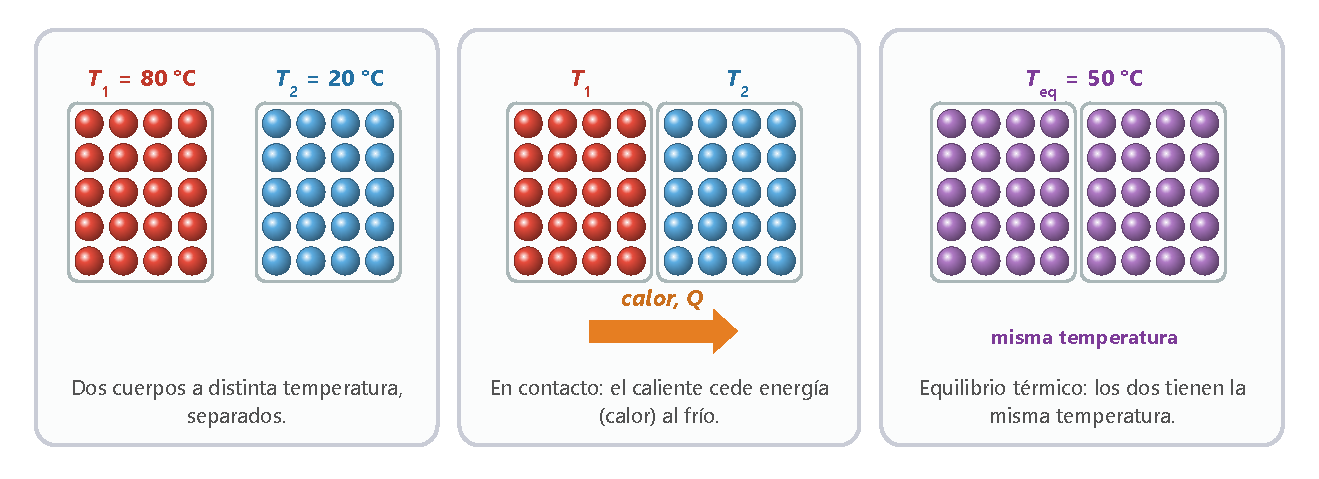
\includegraphics[width=0.85\textwidth]{images/UD13/equilibrio_termico}
    \caption{Dos cuerpos en contacto alcanzan el equilibrio térmico.}
    \label{fig:ud13-equilibrio}
\end{figure}

\begin{definition}[Principio cero de la termodinámica]
    Si dos sistemas A y B están, cada uno por separado, en equilibrio térmico con un tercero C, también están en equilibrio
    térmico entre sí (figura~\ref{fig:ud13-cero}):
    \[ T_A = T_C \ \text{y} \ T_B = T_C \ \Rightarrow \ T_A = T_B \]
\end{definition}

\begin{figure}[H]
    \centering
    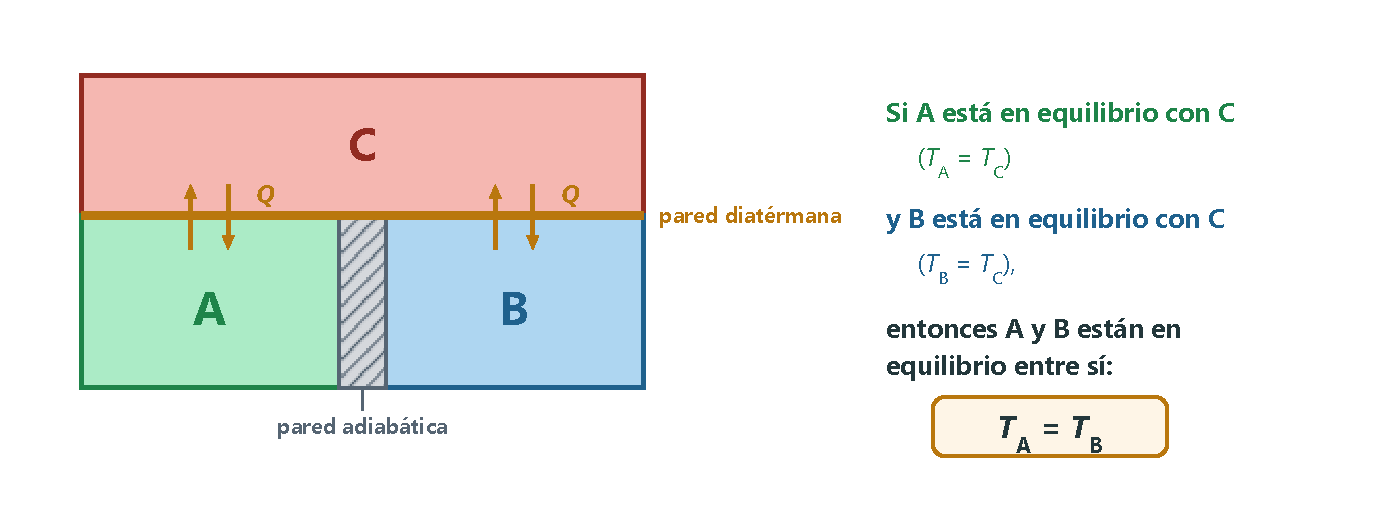
\includegraphics[width=0.8\textwidth]{images/UD13/principio_cero}
    \caption{Principio cero: el equilibrio térmico es transitivo.}
    \label{fig:ud13-cero}
\end{figure}

Parece una obviedad, pero es lo que da sentido a los termómetros: el termómetro es el sistema C, que se pone en equilibrio con
cada cuerpo y nos permite comparar sus temperaturas sin ponerlos en contacto. Se llama «cero» porque se formuló después del
primer y del segundo principio, pero es lógicamente anterior a ellos.

\begin{exercise}
    Después de tres horas en clase, ¿están todos los objetos del aula a la misma temperatura? Entonces, ¿por qué la pata metálica
    de la silla parece más fría que el tablero de madera de la mesa?
    \begin{solu}
        \textcolor{red}{Sí}, si el aula lleva tiempo a temperatura estable, todos han alcanzado el equilibrio térmico con el aire.
        El metal parece más frío porque es \textcolor{red}{mejor conductor} y extrae calor de la mano más deprisa: nuestra
        sensación no mide la temperatura, sino la rapidez con que perdemos calor.
    \end{solu}
\end{exercise}

\begin{exercise}
    ¿Hay equilibrio térmico en estas situaciones? Justifícalo. a) Una bolsa de guisantes que lleva días en el congelador. b) Un
    café que se nos olvidó en la mesa hace dos horas. c) Un cubito de hielo que acabamos de echar a un refresco. d) Una persona
    que nada durante una hora en una piscina.
    \begin{solu}
        a) \textcolor{red}{Sí}, con el interior del congelador. b) \textcolor{red}{Sí}, ya está a la temperatura de la cocina. c)
        \textcolor{red}{No}: el refresco cede calor al hielo. d) \textcolor{red}{No}: el cuerpo regula su temperatura en torno a
        \qty{37}{\degreeCelsius} y cede calor continuamente al agua, más fría.
    \end{solu}
\end{exercise}

\begin{exercise}
    a) La superficie del Sol está a unos \qty{5780}{\kelvin}. Exprésalo en grados Celsius. b) La temperatura más baja medida en la
    Antártida es de \qty{-89.2}{\degreeCelsius}. Exprésala en kelvin.
    \begin{solu}
        a) \(\textcolor{red}{\qty{5507}{\degreeCelsius}}\). b) \(\textcolor{red}{\qty{183.95}{\kelvin}}\) (unos \qty{184}{\kelvin}).
    \end{solu}
\end{exercise}

%========================================================================================
\section{Intercambio de energía en forma de calor}\label{sec:ud13-calor}
%========================================================================================

\subsection{Mecanismos de propagación del calor}

El calor se propaga de tres formas, que suelen darse a la vez (figura~\ref{fig:ud13-mecanismos}):

\begin{itemize}
    \item \textbf{Conducción}: las partículas más agitadas chocan con sus vecinas y les pasan energía cinética, sin que haya
    transporte de materia. Es típica de los sólidos en contacto. Cada material tiene una \textbf{conductividad térmica}: los
    metales son \textbf{buenos conductores}, y el plástico, la madera, el corcho o el aire son \textbf{malos conductores} o
    \textbf{aislantes}.
    \item \textbf{Convección}: la parte caliente de un fluido se dilata, se hace menos densa y asciende, mientras la fría, más
    densa, desciende. Se forman \textbf{corrientes de convección} que transportan materia y energía. Es típica de líquidos y
    gases: las corrientes oceánicas, la brisa marina o el globo aerostático.
    \item \textbf{Radiación}: la energía se transmite mediante \textbf{ondas electromagnéticas}, sobre todo radiación
    \textbf{infrarroja}, y no necesita un medio material: se propaga incluso en el vacío. Así nos llega la energía del Sol, que es
    la principal fuente de energía de la Tierra. Las cámaras termográficas detectan esta radiación.
\end{itemize}

\begin{figure}[H]
    \centering
    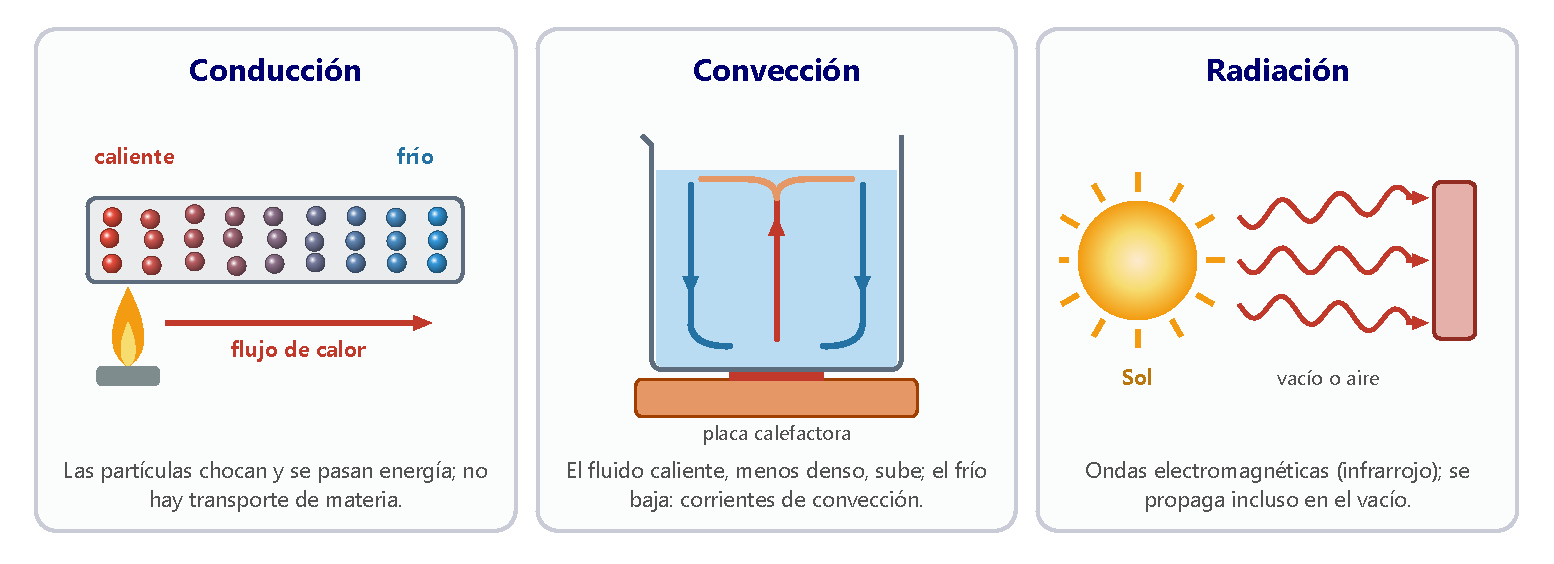
\includegraphics[width=\textwidth]{images/UD13/mecanismos_calor}
    \caption{Mecanismos de propagación del calor.}
    \label{fig:ud13-mecanismos}
\end{figure}

\begin{example}
    \textbf{¿Qué mecanismo es?} Indica el mecanismo de propagación del calor en cada caso: a) se calienta el mango de una cuchara
    metálica dentro de una sopa; b) sentimos el calor de una hoguera en la cara aunque el aire esté frío; c) durante el día, la
    brisa sopla del mar hacia la tierra.

    \textbf{Solución.} a) \textbf{Conducción}: la energía pasa de partícula en partícula a lo largo del metal. b)
    \textbf{Radiación}: la hoguera emite radiación infrarroja, que no necesita calentar el aire. c) \textbf{Convección}: la tierra
    se calienta más que el mar; el aire caliente sobre la tierra sube y su lugar lo ocupa el aire más fresco del mar.
\end{example}

\begin{exercise}
    ¿Qué mecanismo de propagación del calor predomina en cada caso? a) Un radiador calienta una habitación. b) Planchamos una
    camisa. c) Un panel solar térmico calienta agua. d) Las corrientes del océano Atlántico. e) Nos quemamos al tocar una sartén.
    \begin{solu}
        a) \textcolor{red}{Convección} (y algo de radiación). b) \textcolor{red}{Conducción}. c) \textcolor{red}{Radiación} (y
        convección del agua dentro del circuito). d) \textcolor{red}{Convección}. e) \textcolor{red}{Conducción}.
    \end{solu}
\end{exercise}

\begin{exercise}
    ¿Por qué los aparatos de aire acondicionado se colocan en lo alto de las paredes y los radiadores, cerca del suelo?
    \begin{solu}
        Por la \textcolor{red}{convección}: el aire frío, más denso, desciende desde el aparato y enfría toda la habitación; el aire
        caliente del radiador, menos denso, sube y se forman corrientes que reparten el calor.
    \end{solu}
\end{exercise}

\subsection{Calor y variación de temperatura}

Si suministramos la misma cantidad de calor a dos cuerpos de igual masa, sus temperaturas no aumentan lo mismo. La
\textbf{capacidad calorífica} \(C\) de un cuerpo es el calor que necesita para que su temperatura suba \qty{1}{\kelvin}:
\[ C = \frac{Q}{\Delta T} \qquad \text{(en \unit{\joule\per\kelvin})} \]
Depende de la \textbf{masa} y de la \textbf{naturaleza} del material, \(C = m\,c_e\), donde \(c_e\) es el calor específico.

\begin{definition}[Calor específico]
    El \textbf{calor específico} \(c_e\) de una sustancia es el calor que hay que transferir a la unidad de masa para que su
    temperatura aumente \qty{1}{\kelvin}. Se mide en \unit{\joule\per\kg\per\kelvin}, aunque es muy habitual
    \unit{\calorie\per\g\per\degreeCelsius}. El calor intercambiado al variar la temperatura es:
    \[ Q = m\,c_e\,\Delta T = m\,c_e\,(T_f - T_i) \]
\end{definition}

Si \(T_f > T_i\), \(Q > 0\) (el cuerpo absorbe calor); si \(T_f < T_i\), \(Q < 0\) (lo cede). Cuanto mayor es el calor específico,
más energía hace falta para calentar la sustancia y más tarda en enfriarse. El agua tiene un calor específico muy alto
(tabla~\ref{tab:ud13-calor-especifico}): por eso los mares suavizan el clima de las zonas costeras y el agua se usa para
refrigerar motores.

\begin{table}[H]
    \centering
    \caption{Calor específico de algunas sustancias (a \qty{25}{\degreeCelsius} y \qty{1}{\atm})}
    \vspace{-5pt}
    \begin{tabular}{@{}lcc@{}}
        \toprule
        \textbf{Sustancia} & \makecell{\(c_e\) \\ (\unit{\joule\per\kg\per\kelvin})} & \makecell{\(c_e\) \\ (\unit{\calorie\per\g\per\degreeCelsius})} \\
        \midrule
        Agua (líquida) & 4180 & 1 \\[3pt]
        Hielo & 2090 & \num{0.50} \\[3pt]
        Vapor de agua & 2010 & \num{0.48} \\[3pt]
        Etanol & 2420 & \num{0.58} \\[3pt]
        Aluminio & 900 & \num{0.215} \\[3pt]
        Vidrio & 840 & \num{0.20} \\[3pt]
        Hierro & 460 & \num{0.11} \\[3pt]
        Cobre & 385 & \num{0.093} \\[3pt]
        Plata & 234 & \num{0.056} \\[3pt]
        Plomo & 130 & \num{0.031} \\
        \bottomrule
    \end{tabular}
    \label{tab:ud13-calor-especifico}
\end{table}

\begin{remark}
    El calor específico no es una función de estado, porque depende de cómo se caliente la sustancia. En los gases se distingue
    el calor específico molar \textbf{a presión constante}, \(c_p\), y \textbf{a volumen constante}, \(c_v\), y se usa el mol como
    cantidad de materia: \(Q = n\,c_{p}\,\Delta T\) o \(Q = n\,c_{v}\,\Delta T\), con \(c\) en \unit{\joule\per\mol\per\kelvin}.
\end{remark}

\begin{example}
    \textbf{Agua para un té.} a) ¿Qué calor hay que suministrar a \qty{300}{\g} de agua para calentarla de \qty{20}{\degreeCelsius} a
    \qty{90}{\degreeCelsius}? Exprésalo en julios y en kilocalorías. b) ¿Qué calor pierden \qty{500}{\g} de agua al enfriarse en
    la nevera de \qty{30}{\degreeCelsius} a \qty{5}{\degreeCelsius}?

    \textbf{Solución.} a) \(Q = m\,c_e\,\Delta T = \num{0.300} \cdot 4180 \cdot (90 - 20) = \qty{8.78e4}{\joule} = \qty{87.8}{\kilo\joule}\).
    En calorías: \(Q = 300 \cdot 1 \cdot 70 = \qty{21000}{\calorie} = \qty{21}{\kilo\calorie}\).

    b) \(Q = \num{0.500} \cdot 4180 \cdot (5 - 30) = \qty{-5.23e4}{\joule} = \qty{-52.3}{\kilo\joule}\). El signo negativo indica
    que el agua cede calor.
\end{example}

\begin{exercise}
    Se suministran \qty{1500}{\calorie} a \qty{250}{\g} de cobre que están a \qty{18}{\degreeCelsius}. ¿Qué temperatura alcanza?
    \begin{solu}
        \(\Delta T = \dfrac{Q}{m\,c_e} = \dfrac{1500}{250 \cdot \num{0.093}} = \qty{64.5}{\degreeCelsius}\);
        \(T_f = \textcolor{red}{\qty{82.5}{\degreeCelsius}}\).
    \end{solu}
\end{exercise}

\begin{exercise}
    ¿Qué calor hay que suministrar a una pieza de hierro de \qty{800}{\kg} para calentarla desde \qty{20}{\degreeCelsius} hasta
    \qty{1200}{\degreeCelsius} para forjarla? Exprésalo en kilocalorías y en julios.
    \begin{solu}
        \(Q = \num{8e5}~\mathrm{g} \cdot \num{0.11} \cdot 1180 = \qty{1.04e8}{\calorie} = \textcolor{red}{\qty{1.04e5}{\kilo\calorie}}
        = \textcolor{red}{\qty{4.34e8}{\joule}}\).
    \end{solu}
\end{exercise}

\paragraph{Equilibrio térmico y calorimetría.} Si mezclamos dos cuerpos a distinta temperatura en un recipiente aislado
(\textbf{calorímetro}), el calor que cede el caliente lo absorbe el frío, hasta que ambos alcanzan la misma temperatura final
\(T_{eq}\) (figura~\ref{fig:ud13-calorimetro}). Como no se pierde energía:
\[ Q_{\text{cedido}} + Q_{\text{absorbido}} = 0 \ \Rightarrow \ m_1\,c_1\,(T_{eq} - T_1) + m_2\,c_2\,(T_{eq} - T_2) = 0 \]

\begin{figure}[H]
    \centering
    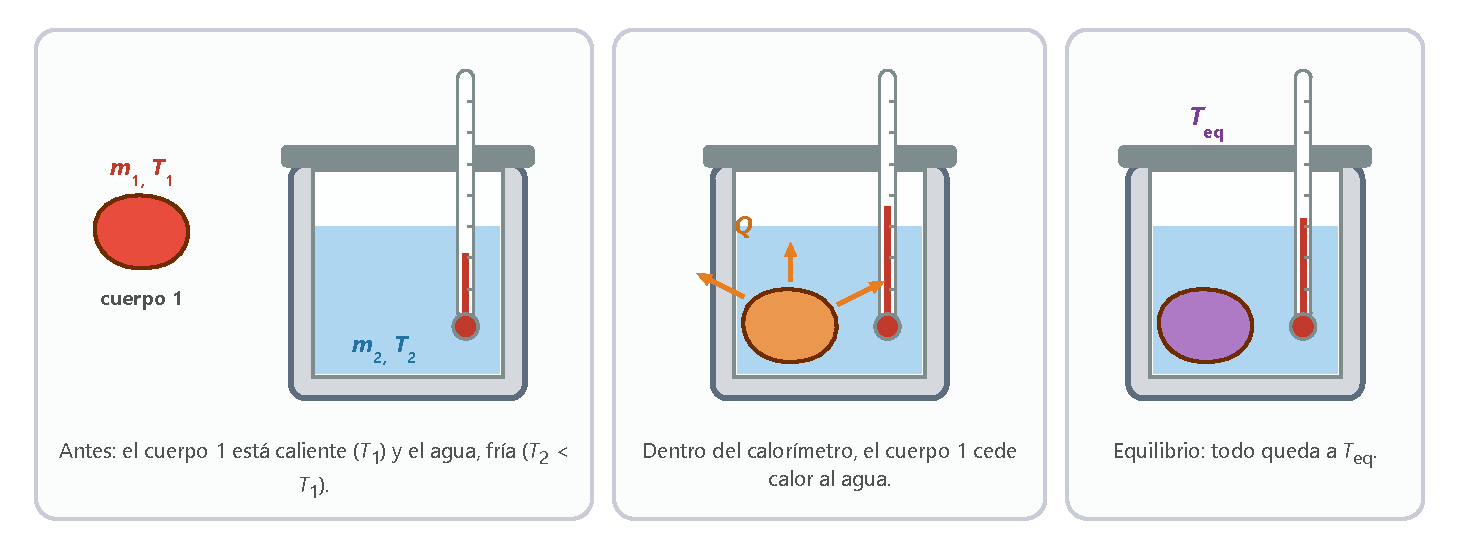
\includegraphics[width=0.85\textwidth]{images/UD13/balance_calorimetro}
    \caption{En un calorímetro, el calor cedido por el cuerpo caliente lo absorbe el agua.}
    \label{fig:ud13-calorimetro}
\end{figure}

\begin{example}
    \textbf{Templar el agua del baño.} Se mezclan \qty{1.2}{\litre} de agua a \qty{15}{\degreeCelsius} con \qty{0.8}{\litre} de
    agua a \qty{70}{\degreeCelsius} en un recipiente aislado. Calcula la temperatura final y el calor que intercambia cada parte.
    Densidad del agua: \qty{1}{\kg\per\litre}.

    \textbf{Solución.} Las masas son \qty{1.2}{\kg} y \qty{0.8}{\kg}. Como el calor específico es el mismo, se simplifica:
    \[ \num{1.2}\,(T - 15) + \num{0.8}\,(T - 70) = 0 \Rightarrow T = \frac{\num{1.2} \cdot 15 + \num{0.8} \cdot 70}{2} = \qty{37}{\degreeCelsius} \]
    Agua fría: \(Q_1 = \num{1.2} \cdot 4180 \cdot (37 - 15) = \qty{+1.10e5}{\joule}\) (absorbe). Agua caliente: \(Q_2 =
    \num{0.8} \cdot 4180 \cdot (37 - 70) = \qty{-1.10e5}{\joule}\) (cede la misma cantidad).
\end{example}

\begin{exercise}
    Se mezclan \qty{5}{\kg} de agua a \qty{80}{\degreeCelsius} con \qty{10}{\kg} de agua a \qty{20}{\degreeCelsius}. ¿Cuál es la
    temperatura final? ¿Qué calor cede el agua caliente?
    \begin{solu}
        \(T = \dfrac{5 \cdot 80 + 10 \cdot 20}{15} = \textcolor{red}{\qty{40}{\degreeCelsius}}\);
        \(Q = 5 \cdot 4180 \cdot (40 - 80) = \textcolor{red}{\qty{-8.36e5}{\joule}}\).
    \end{solu}
\end{exercise}

\subsection{Cambios de estado}

Mientras una sustancia pura cambia de estado, su temperatura \textbf{no varía} aunque le sigamos dando calor: toda la energía se
emplea en vencer las fuerzas entre las partículas. Los cambios de estado son procesos \textbf{isotérmicos} y reversibles: la energía
absorbida en un sentido (por ejemplo, al fundir) es la misma que se cede en el sentido contrario (al solidificar)
(figura~\ref{fig:ud13-cambios}).

\begin{figure}[H]
    \centering
    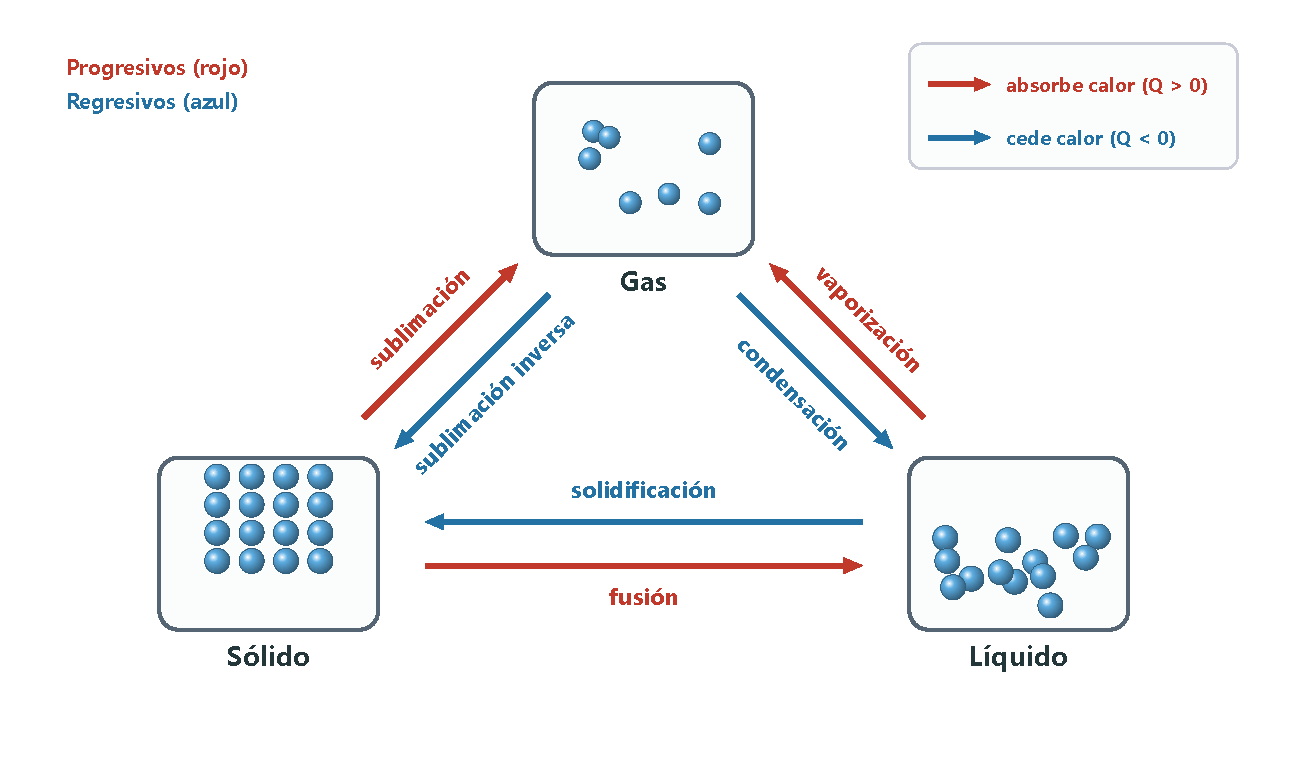
\includegraphics[width=0.8\textwidth]{images/UD13/cambios_estado}
    \caption{Cambios de estado progresivos (absorben calor) y regresivos (lo ceden).}
    \label{fig:ud13-cambios}
\end{figure}

\begin{definition}[Calor latente]
    El \textbf{calor latente} \(L\) de un cambio de estado es la energía que hay que suministrar a la unidad de masa de una
    sustancia para que cambie de estado a temperatura y presión constantes. Hay calor latente de \textbf{fusión} \(L_f\), de
    \textbf{vaporización} \(L_v\) y de \textbf{sublimación} \(L_s\). Se mide en \unit{\joule\per\kg} (también en
    \unit{\calorie\per\g}). El calor intercambiado es:
    \[ |Q| = m\,L \]
\end{definition}

En un cambio \textbf{progresivo} (fusión, vaporización, sublimación) el sistema absorbe energía, \(Q > 0\); en uno
\textbf{regresivo} (solidificación, condensación, sublimación inversa) la cede, \(Q < 0\).

\begin{table}[H]
    \centering
    \caption{Temperaturas de cambio de estado (a \qty{1}{\atm}) y calores latentes}
    \vspace{-5pt}
    \begin{tabular}{@{}lcccc@{}}
        \toprule
        \textbf{Sustancia} & \makecell{\textbf{Fusión} \\ (\unit{\degreeCelsius})} & \makecell{\(L_f\) \\ (\unit{\kilo\joule\per\kg})} &
        \makecell{\textbf{Ebullición} \\ (\unit{\degreeCelsius})} & \makecell{\(L_v\) \\ (\unit{\kilo\joule\per\kg})} \\
        \midrule
        Agua & 0 & 334 & 100 & 2260 \\[3pt]
        Etanol & \num{-114} & 104 & 78 & 854 \\[3pt]
        Mercurio & \num{-39} & 11 & 357 & 296 \\[3pt]
        Plomo & 327 & 25 & 1750 & 871 \\[3pt]
        Hierro & 1538 & 247 & 2862 & 6090 \\
        \bottomrule
    \end{tabular}
    \label{tab:ud13-latentes}
\end{table}

\begin{example}
    \textbf{Del congelador al vapor.} Calcula la energía necesaria para transformar \qty{200}{\g} de hielo a \qty{-10}{\degreeCelsius}
    en vapor de agua a \qty{100}{\degreeCelsius}. Datos: \(c_{\text{hielo}} = \qty{2090}{\joule\per\kg\per\kelvin}\),
    \(c_{\text{agua}} = \qty{4180}{\joule\per\kg\per\kelvin}\), \(L_f = \qty{3.34e5}{\joule\per\kg}\), \(L_v = \qty{2.26e6}{\joule\per\kg}\).

    \textbf{Solución.} Hay cuatro etapas (figura~\ref{fig:ud13-calentamiento}):

    1. Calentar el hielo hasta \qty{0}{\degreeCelsius}: \(Q_1 = \num{0.2} \cdot 2090 \cdot 10 = \qty{4180}{\joule}\).

    2. Fundir el hielo: \(Q_2 = \num{0.2} \cdot \num{3.34e5} = \qty{66800}{\joule}\).

    3. Calentar el agua hasta \qty{100}{\degreeCelsius}: \(Q_3 = \num{0.2} \cdot 4180 \cdot 100 = \qty{83600}{\joule}\).

    4. Vaporizar el agua: \(Q_4 = \num{0.2} \cdot \num{2.26e6} = \qty{452000}{\joule}\).

    En total, \(Q = Q_1 + Q_2 + Q_3 + Q_4 = \qty{6.07e5}{\joule} = \qty{607}{\kilo\joule}\). Fíjate en que la vaporización se lleva
    tres cuartas partes de la energía.
\end{example}

\begin{figure}[H]
    \centering
    \begin{tikzpicture}
        \begin{axis}[grafica, width=0.75\linewidth, height=6cm, xlabel={Calor suministrado (kJ)}, ylabel={\(t\) (\unit{\degreeCelsius})},
            xmin=0, xmax=650, ymin=-20, ymax=130, xtick={0,4.2,71,154.6,606.6}, xticklabels={0,,71,155,607},
            ytick={-10,0,100}]
            \addplot[very thick, ocre] coordinates {(0,-10) (4.18,0) (70.98,0) (154.58,100) (606.58,100) (630,112)};
            \node[font=\scriptsize, anchor=south] at (axis cs:37,2) {fusión};
            \node[font=\scriptsize, anchor=south, align=center] at (axis cs:380,102) {ebullición (agua + vapor)};
            \node[font=\scriptsize, anchor=west] at (axis cs:118,40) {agua};
            \node[font=\scriptsize, anchor=west] at (axis cs:8,-10) {hielo};
            \node[font=\scriptsize, anchor=south east] at (axis cs:640,112) {vapor};
        \end{axis}
    \end{tikzpicture}
    \caption{Curva de calentamiento de \qty{200}{\g} de hielo: durante los cambios de estado la temperatura no varía.}
    \label{fig:ud13-calentamiento}
\end{figure}

\begin{exercise}
    ¿Qué energía hay que suministrar para vaporizar \qty{80}{\g} de agua que ya está a \qty{100}{\degreeCelsius}?
    \(L_v = \qty{540}{\calorie\per\g}\).
    \begin{solu}
        \(Q = m\,L_v = 80 \cdot 540 = \textcolor{red}{\qty{43200}{\calorie}} = \qty{43.2}{\kilo\calorie} \approx \qty{181}{\kilo\joule}\).
    \end{solu}
\end{exercise}

\begin{exercise}
    ¿Por qué una quemadura con vapor de agua a \qty{100}{\degreeCelsius} es más grave que una con agua líquida a
    \qty{100}{\degreeCelsius}?
    \begin{solu}
        Porque el vapor, al condensarse sobre la piel, cede además su \textcolor{red}{calor latente de vaporización} (unos
        \qty{2260}{\joule} por gramo), que es mucho mayor que el calor que cede el agua al enfriarse.
    \end{solu}
\end{exercise}

\subsection{Dilatación térmica}

Al calentar un cuerpo, sus partículas se agitan más y se separan: aumentan sus dimensiones. Es la \textbf{dilatación térmica}; el
proceso contrario es la \textbf{contracción}. Según las dimensiones que importan, distinguimos (tabla~\ref{tab:ud13-dilatacion}):

\begin{table}[H]
    \centering
    \caption{Tipos de dilatación}
    \vspace{-5pt}
    \begin{tabular}{@{}lL{4.3cm}cL{4.4cm}@{}}
        \toprule
        \textbf{Dilatación} & \textbf{Se da en\dots} & \textbf{Expresión} & \textbf{Coeficiente} \\
        \midrule
        Lineal & varillas, cables, raíles (domina la longitud) & \(L = L_0\,(1 + \lambda\,\Delta T)\) & \(\lambda\), dilatación
        lineal \\[3pt]
        Superficial & placas y láminas & \(S = S_0\,(1 + \beta\,\Delta T)\) & \(\beta \approx 2\lambda\), dilatación superficial \\[3pt]
        Cúbica & cuerpos con tres dimensiones, líquidos y gases & \(V = V_0\,(1 + \gamma\,\Delta T)\) & \(\gamma \approx 3\lambda\),
        dilatación cúbica \\
        \bottomrule
    \end{tabular}
    \label{tab:ud13-dilatacion}
\end{table}

Los coeficientes de dilatación son característicos de cada material y se miden en \unit{\per\kelvin} (o
\unit{\per\degreeCelsius}): son el aumento relativo de longitud, superficie o volumen por cada grado. Los gases se dilatan mucho
más que los líquidos, y estos más que los sólidos. \textbf{Gay-Lussac} comprobó que, a presión constante, todos los gases tienen
prácticamente el mismo coeficiente: \(\gamma \approx \frac{1}{273}~\unit{\per\degreeCelsius}\).

\begin{figure}[H]
    \centering
    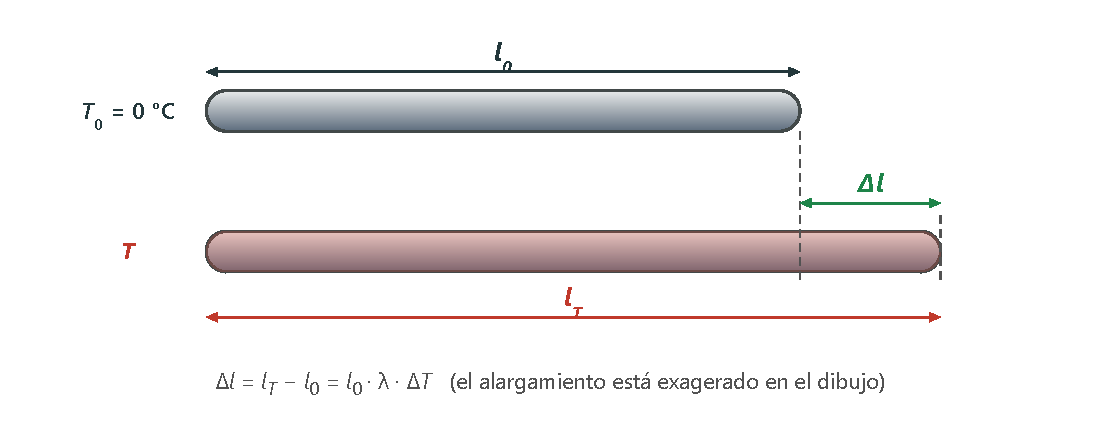
\includegraphics[width=0.65\textwidth]{images/UD13/dilatacion}
    \caption{Dilatación lineal de una barra.}
    \label{fig:ud13-dilatacion}
\end{figure}

La dilatación se tiene en cuenta en ingeniería: los puentes y las vías tienen \textbf{juntas de dilatación}, y los cables del
tendido eléctrico se cuelgan algo flojos para que no se rompan al contraerse en invierno. Los termostatos de muchos aparatos
usan una \textbf{lámina bimetálica}, dos metales soldados que se dilatan distinto: al calentarse se curva y abre o cierra un
circuito (figura~\ref{fig:ud13-bimetal}).

\begin{figure}[H]
    \centering
    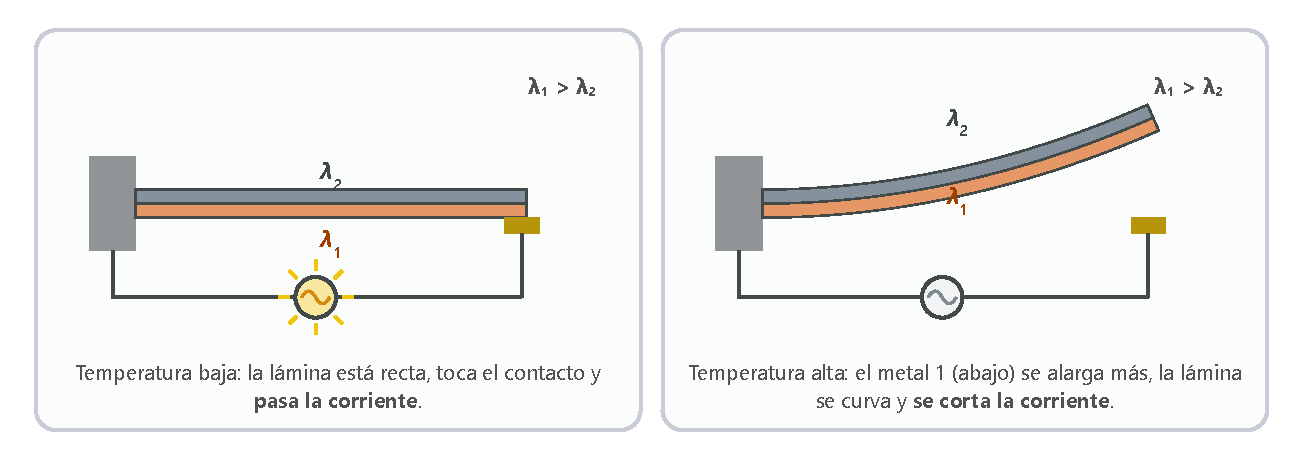
\includegraphics[width=0.85\textwidth]{images/UD13/bimetal}
    \caption{Termostato de lámina bimetálica.}
    \label{fig:ud13-bimetal}
\end{figure}

\begin{example}
    \textbf{Juntas en las vías.} Un raíl de acero mide \qty{25}{\m} a \qty{10}{\degreeCelsius}. ¿Cuánto se alarga un día de verano en
    que alcanza \qty{45}{\degreeCelsius}? \(\lambda_{\text{acero}} = \qty{1.2e-5}{\per\kelvin}\).

    \textbf{Solución.} \(\Delta L = L_0\,\lambda\,\Delta T = 25 \cdot \num{1.2e-5} \cdot (45 - 10) = \qty{1.05e-2}{\m} =
    \qty{10.5}{\mm}\). Por eso se deja un hueco de algo más de un centímetro entre raíles.
\end{example}

\begin{exercise}
    Una barra de aluminio mide \qty{3}{\m} a \qty{20}{\degreeCelsius}. ¿Cuánto se alarga si se calienta hasta \qty{180}{\degreeCelsius}?
    \(\lambda = \qty{2.4e-5}{\per\kelvin}\).
    \begin{solu}
        \(\Delta L = 3 \cdot \num{2.4e-5} \cdot 160 = \qty{1.15e-2}{\m} = \textcolor{red}{\qty{11.5}{\mm}}\).
    \end{solu}
\end{exercise}

%========================================================================================
\section{Intercambio de energía en forma de trabajo}\label{sec:ud13-trabajo}
%========================================================================================

El \textbf{trabajo termodinámico} es la energía que intercambian el sistema y el entorno sin que intervenga una diferencia de
temperatura. Suele ir asociado a una fuerza que produce un desplazamiento en el sistema: en un gas, al cambiar su volumen.

\subsection{Trabajo de expansión o compresión de un gas}

Imaginemos un gas encerrado en un cilindro con un émbolo de superficie \(S\) que puede moverse sin rozamiento, sometido a una
presión exterior constante \(p\) (figura~\ref{fig:ud13-embolo}). Si calentamos el gas, sus partículas chocan con más energía
contra el émbolo, lo empujan y el gas se expande: el émbolo sube \(\Delta h\) y el volumen aumenta \(\Delta V = S\,\Delta h\).

\begin{figure}[H]
    \centering
    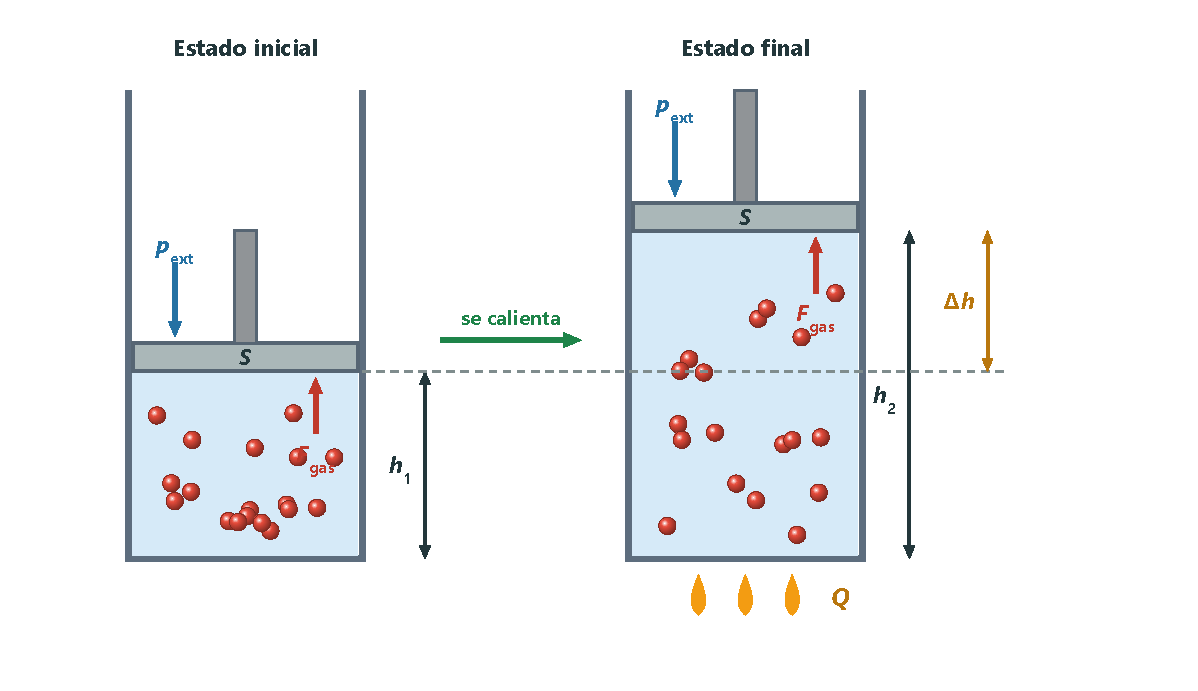
\includegraphics[width=0.7\textwidth]{images/UD13/expansion_embolo}
    \caption{Expansión de un gas a presión constante.}
    \label{fig:ud13-embolo}
\end{figure}

La fuerza que vence el gas es \(F = p\,S\), y con nuestro criterio de signos el trabajo de expansión es negativo (el sistema
pierde energía):
\[ W = -F\,\Delta h = -p\,S\,\Delta h = -p\,\Delta V = -p\,(V_f - V_i) \]

\begin{table}[H]
    \centering
    \caption{Signo del trabajo de un gas}
    \vspace{-5pt}
    \begin{tabular}{@{}lcL{9.5cm}@{}}
        \toprule
        \textbf{Proceso} & \textbf{Signo} & \textbf{Descripción} \\
        \midrule
        Expansión & \(W < 0\) & \(\Delta V > 0\): el gas realiza trabajo sobre el entorno y pierde energía. \\[3pt]
        Compresión & \(W > 0\) & \(\Delta V < 0\): el entorno realiza trabajo sobre el gas y le comunica energía. \\[3pt]
        Volumen constante & \(W = 0\) & \(\Delta V = 0\): no hay trabajo de expansión ni de compresión. \\
        \bottomrule
    \end{tabular}
    \label{tab:ud13-signo-trabajo}
\end{table}

\begin{remark}
    Para que el trabajo salga en julios, la presión debe ir en pascales y el volumen en metros cúbicos:
    \(\qty{1}{\litre} = \qty{e-3}{\m\cubed}\) y \(\qty{1}{\cm\cubed} = \qty{e-6}{\m\cubed}\). También es útil saber que
    \(\qty{1}{\atm\litre} = \qty{101.3}{\joule}\).
\end{remark}

\begin{example}
    \textbf{Expansión contra la presión exterior.} Un gas encerrado en un cilindro de paredes adiabáticas con un émbolo móvil ocupa
    \qty{3}{\litre}. Se expande hasta \qty{8}{\litre} contra una presión exterior constante de \qty{150}{\kilo\pascal}. ¿Qué trabajo
    se realiza?

    \textbf{Solución.} \(W = -p\,(V_f - V_i) = -\num{1.5e5} \cdot (8 - 3) \cdot \num{e-3} = \qty{-750}{\joule}\). Es negativo porque
    el gas hace trabajo sobre el entorno.
\end{example}

\begin{exercise}
    Si el gas del ejemplo anterior se comprimiera de \qty{6}{\litre} a \qty{2}{\litre} a una presión de \qty{120}{\kilo\pascal}, ¿qué
    trabajo se realizaría? ¿Y si el proceso fuera isocórico?
    \begin{solu}
        \(W = -\num{1.2e5} \cdot (2 - 6) \cdot \num{e-3} = \textcolor{red}{\qty{+480}{\joule}}\). En un proceso isocórico,
        \(\Delta V = 0\) y \(W = \textcolor{red}{0}\).
    \end{solu}
\end{exercise}

\begin{exercise}
    Calcula el trabajo realizado al comprimir un gas desde \qty{800}{\cm\cubed} hasta \qty{300}{\cm\cubed} con una presión exterior
    de \qty{250}{\kilo\pascal}.
    \begin{solu}
        \(W = -\num{2.5e5} \cdot (300 - 800) \cdot \num{e-6} = \textcolor{red}{\qty{+125}{\joule}}\).
    \end{solu}
\end{exercise}

\subsection{Diagramas \texorpdfstring{\(p\)-\(V\)}{p-V}}

Los procesos de un gas se representan en un diagrama \(p\)-\(V\), con el volumen en abscisas y la presión en ordenadas. En un
proceso isobárico, la gráfica es una recta horizontal y \(|W| = p\,\Delta V\) es el área del rectángulo bajo ella. Esta idea se
generaliza a cualquier proceso:

\begin{definition}[Interpretación gráfica del trabajo]
    El \textbf{valor absoluto del trabajo} intercambiado en un proceso es el \textbf{área} comprendida entre la gráfica \(p = p(V)\) y
    el eje de abscisas, entre \(V_i\) y \(V_f\). El signo es negativo si el volumen aumenta y positivo si disminuye.
\end{definition}

\begin{figure}[H]
    \centering
    \begin{tikzpicture}
        \begin{axis}[grafica, width=0.36\linewidth, height=4.4cm, xlabel={\(V\)}, ylabel={\(p\)}, xmin=0, xmax=6, ymin=0, ymax=5,
            xtick={1.2,4.8}, xticklabels={\(V_A\),\(V_B\)}, ytick=\empty, title={\small Isobárico}]
            \addplot[fill=ocre!25, draw=none] coordinates {(1.2,0) (1.2,3) (4.8,3) (4.8,0)} \closedcycle;
            \addplot[very thick, ocre, -latex] coordinates {(1.2,3) (4.8,3)};
            \node[font=\small] at (axis cs:3,1.5) {\(W = -p\,\Delta V\)};
            \node[font=\small, anchor=south] at (axis cs:1.2,3) {A};
            \node[font=\small, anchor=south] at (axis cs:4.8,3) {B};
        \end{axis}
    \end{tikzpicture}\hfill
    \begin{tikzpicture}
        \begin{axis}[grafica, width=0.36\linewidth, height=4.4cm, xlabel={\(V\)}, ylabel={\(p\)}, xmin=0, xmax=6, ymin=0, ymax=5,
            xtick={1.2,4.8}, xticklabels={\(V_A\),\(V_B\)}, ytick=\empty, title={\small Isotérmico}]
            \addplot[fill=ocre!25, draw=none, domain=1.2:4.8] {5/x} \closedcycle;
            \addplot[thick, gray, dashed, domain=1.05:5.8] {5/x};
            \addplot[very thick, ocre, domain=1.2:4.8] {5/x};
            \node[font=\small] at (axis cs:2.9,0.8) {\(W\)};
            \node[font=\small, anchor=south west] at (axis cs:1.2,4.17) {A};
            \node[font=\small, anchor=south west] at (axis cs:4.8,1.04) {B};
        \end{axis}
    \end{tikzpicture}\hfill
    \begin{tikzpicture}
        \begin{axis}[grafica, width=0.36\linewidth, height=4.4cm, xlabel={\(V\)}, ylabel={\(p\)}, xmin=0, xmax=6, ymin=0, ymax=5,
            xtick={3}, xticklabels={\(V\)}, ytick=\empty, title={\small Isocórico}]
            \addplot[very thick, ocre, -latex] coordinates {(3,1.2) (3,4)};
            \addplot[thin, gray, dashed] coordinates {(0,1.2) (3,1.2)};
            \addplot[thin, gray, dashed] coordinates {(0,4) (3,4)};
            \node[font=\small, anchor=west] at (axis cs:3,1.2) {A};
            \node[font=\small, anchor=west] at (axis cs:3,4) {B};
            \node[font=\small] at (axis cs:4.5,2.6) {\(W = 0\)};
        \end{axis}
    \end{tikzpicture}
    \caption{Trabajo en los diagramas \(p\)-\(V\): es el área bajo la gráfica.}
    \label{fig:ud13-diagramas}
\end{figure}

\begin{itemize}
    \item \textbf{Isobárico}: recta horizontal; \(W = -p\,(V_B - V_A)\).
    \item \textbf{Isotérmico}: según la ley de Boyle, \(p = n\,R\,T/V\), la gráfica es una hipérbola. El cálculo del área (con una
    integral, que estudiarás en Matemáticas) da:
    \[ W = -n\,R\,T \ln\frac{V_B}{V_A} \]
    \item \textbf{Isocórico}: recta vertical; el área es nula y \(W = 0\).
\end{itemize}

Si el sistema recorre un \textbf{ciclo} (vuelve al estado inicial), el trabajo total es el \textbf{área encerrada} por el ciclo:
es negativo (el gas hace trabajo neto) si el ciclo se recorre en sentido horario, y positivo si se recorre en sentido antihorario.

\begin{example}
    \textbf{Trabajo en un ciclo.} Un gas recorre el ciclo de la figura~\ref{fig:ud13-ciclo}: 1 (\qty{1.5}{\litre},
    \qty{250}{\kilo\pascal}) \(\rightarrow\) 2 (\qty{5.5}{\litre}, \qty{250}{\kilo\pascal}) \(\rightarrow\) 3 (\qty{5.5}{\litre},
    \qty{100}{\kilo\pascal}) \(\rightarrow\) 4 (\qty{1.5}{\litre}, \qty{100}{\kilo\pascal}) \(\rightarrow\) 1. Calcula el trabajo en
    cada tramo y en el ciclo completo.

    \textbf{Solución.} Tramos isocóricos (2 \(\rightarrow\) 3 y 4 \(\rightarrow\) 1): \(W = 0\). Tramos isobáricos:
    \begin{gather*}
        W_{1\to2} = -\num{2.5e5} \cdot (\num{5.5} - \num{1.5}) \cdot \num{e-3} = \qty{-1000}{\joule} \\
        W_{3\to4} = -\num{1.0e5} \cdot (\num{1.5} - \num{5.5}) \cdot \num{e-3} = \qty{+400}{\joule}
    \end{gather*}
    \(W_{\text{ciclo}} = -1000 + 0 + 400 + 0 = \qty{-600}{\joule}\). Coincide con el área del rectángulo,
    \((250 - 100)\,\unit{\kilo\pascal} \cdot \qty{4}{\litre} = \qty{600}{\joule}\), con signo negativo porque se recorre en sentido
    horario: el gas realiza trabajo neto sobre el entorno.
\end{example}

\begin{figure}[H]
    \centering
    \begin{tikzpicture}
        \begin{axis}[grafica, width=0.5\linewidth, height=5cm, xlabel={\(V\) (L)}, ylabel={\(p\) (kPa)}, xmin=0, xmax=7, ymin=0,
            ymax=300, xtick={1.5,5.5}, ytick={100,250}]
            \addplot[fill=ocre!20, draw=none] coordinates {(1.5,100) (1.5,250) (5.5,250) (5.5,100)} -- cycle;
            \addplot[very thick, ocre, -latex] coordinates {(1.5,250) (3.6,250)};
            \addplot[very thick, ocre, -latex] coordinates {(3.5,250) (5.5,250) (5.5,170)};
            \addplot[very thick, ocre, -latex] coordinates {(5.5,180) (5.5,100) (3.4,100)};
            \addplot[very thick, ocre, -latex] coordinates {(3.5,100) (1.5,100) (1.5,180)};
            \addplot[very thick, ocre] coordinates {(1.5,175) (1.5,250)};
            \node[font=\small, anchor=south east] at (axis cs:1.5,250) {1};
            \node[font=\small, anchor=south west] at (axis cs:5.5,250) {2};
            \node[font=\small, anchor=north west] at (axis cs:5.5,100) {3};
            \node[font=\small, anchor=north east] at (axis cs:1.5,100) {4};
        \end{axis}
    \end{tikzpicture}
    \caption{Ciclo rectangular en un diagrama \(p\)-\(V\).}
    \label{fig:ud13-ciclo}
\end{figure}

\begin{example}
    \textbf{Expansión isotérmica.} \qty{0.20}{\mol} de un gas ideal a \qty{27}{\degreeCelsius} se expanden de forma isotérmica desde
    \qty{2.0}{\litre} hasta \qty{5.0}{\litre}. ¿Qué trabajo se realiza?

    \textbf{Solución.} \(T = \qty{300}{\kelvin}\):
    \(W = -n\,R\,T\ln\dfrac{V_B}{V_A} = -\num{0.20} \cdot \num{8.31} \cdot 300 \cdot \ln\dfrac{5}{2} = \qty{-457}{\joule}\).
\end{example}

\begin{exercise}
    Representa en un diagrama \(p\)-\(V\) un proceso isocórico, uno isobárico y uno isotérmico, e indica en cuál de ellos es nulo el
    trabajo.
    \begin{solu}
        Isocórico: recta vertical; isobárico: recta horizontal; isotérmico: rama de hipérbola. El trabajo es nulo en el
        \textcolor{red}{isocórico}.
    \end{solu}
\end{exercise}

\begin{exercise}
    Un gas recorre el ciclo triangular 1 (\qty{2}{\litre}, \qty{300}{\kilo\pascal}) \(\rightarrow\) 2 (\qty{8}{\litre},
    \qty{100}{\kilo\pascal}) en línea recta \(\rightarrow\) 3 (\qty{2}{\litre}, \qty{100}{\kilo\pascal}) \(\rightarrow\) 1. Calcula el
    trabajo en cada tramo y en el ciclo.
    \begin{solu}
        \(W_{1\to2} = -\dfrac{300 + 100}{2}\,\unit{\kilo\pascal} \cdot \qty{6}{\litre} = \textcolor{red}{\qty{-1200}{\joule}}\) (área del
        trapecio); \(W_{2\to3} = -\num{1e5} \cdot (2 - 8) \cdot \num{e-3} = \textcolor{red}{\qty{+600}{\joule}}\);
        \(W_{3\to1} = \textcolor{red}{0}\). \(W_{\text{ciclo}} = \textcolor{red}{\qty{-600}{\joule}}\) (área del triángulo).
    \end{solu}
\end{exercise}

%========================================================================================
\section{Energía interna y primer principio de la termodinámica}\label{sec:ud13-primer-principio}
%========================================================================================

Las partículas de un sistema tienen energía cinética de traslación, pero también de rotación y de vibración, y energía potencial
debida a las fuerzas entre ellas (figura~\ref{fig:ud13-energia-interna}).

\begin{definition}[Energía interna]
    La \textbf{energía interna} \(U\) de un sistema es la suma de todas las energías de las partículas que lo forman. Es una
    \textbf{función de estado} y se mide en julios.
\end{definition}

\begin{figure}[H]
    \centering
    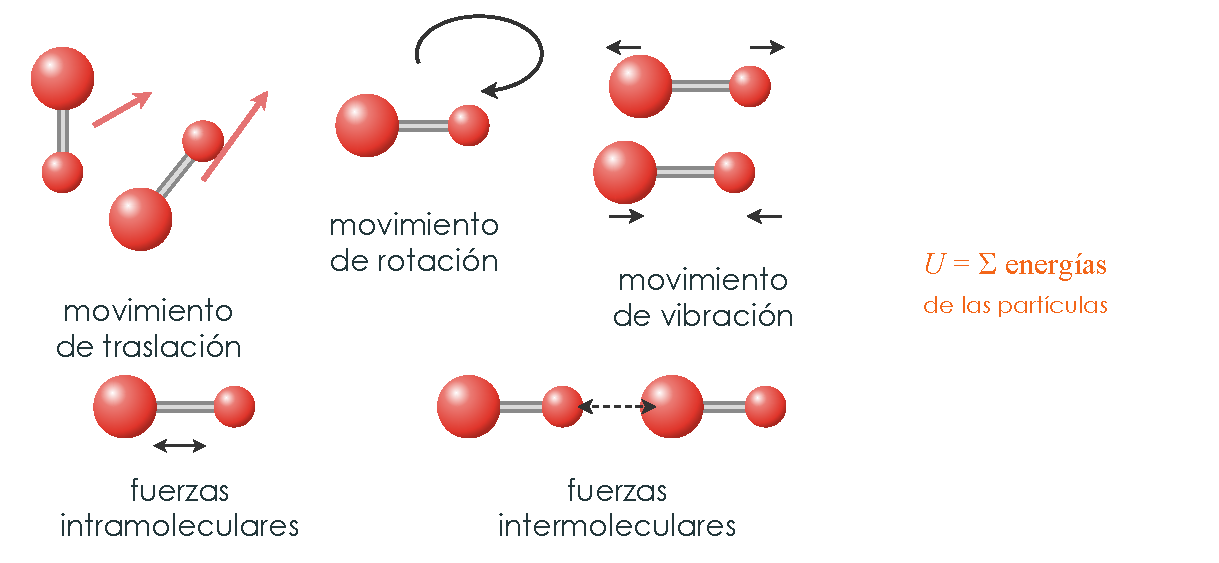
\includegraphics[width=0.7\textwidth]{images/UD13/energia_interna}
    \caption{Contribuciones a la energía interna.}
    \label{fig:ud13-energia-interna}
\end{figure}

No podemos medir la energía de cada partícula, así que no conocemos el valor absoluto de \(U\); pero sí podemos medir su
\textbf{variación}, \(\Delta U\), cuando el sistema pasa de un estado a otro. En un \textbf{gas ideal} no hay fuerzas entre las
partículas y la energía interna depende solo de la temperatura: si \(T\) no cambia, \(U\) tampoco.

\begin{definition}[Primer principio de la termodinámica]
    La variación de la energía interna de un sistema es igual a la suma del calor y del trabajo que intercambia con su entorno:
    \[ \Delta U = Q + W \]
\end{definition}

Es el \textbf{principio de conservación de la energía} aplicado a los sistemas termodinámicos: la energía no se crea ni se
destruye, de modo que si la energía interna de un sistema cambia, es porque ha intercambiado calor o trabajo con el entorno. Lo
enunció \textbf{Rudolf Clausius} en 1850, a partir de los trabajos de Carnot y de Joule.

Con nuestro criterio de signos:
\begin{itemize}
    \item El calor absorbido y el trabajo recibido aumentan \(U\); el calor cedido y el trabajo realizado la disminuyen.
    \item En un \textbf{proceso cíclico}, el sistema vuelve al estado inicial y, como \(U\) es función de estado,
    \(\Delta U = 0\): \(Q = -W\). En un \textbf{sistema aislado}, \(Q = W = 0\) y \(U\) es constante.
\end{itemize}

\begin{table}[H]
    \centering
    \caption{El primer principio en los distintos procesos}
    \vspace{-5pt}
    \begin{tabular}{@{}lcL{7.8cm}@{}}
        \toprule
        \textbf{Proceso} & \textbf{Primer principio} & \textbf{Comentario} \\
        \midrule
        Adiabático & \(\Delta U = W\) & No hay calor; la energía interna cambia solo por el trabajo. En una compresión
        adiabática \(W > 0\) y el gas se calienta. \\[3pt]
        Isocórico & \(\Delta U = Q_V\) & \(W = 0\): todo el calor a volumen constante, \(Q_V\), se invierte en cambiar \(U\). \\[3pt]
        Isobárico & \(\Delta U = Q_p - p\,\Delta V\) & \(Q_p\) es el calor a presión constante. \\[3pt]
        Isotérmico (gas ideal) & \(\Delta U = 0\) & \(T\) no cambia, \(U\) tampoco: \(Q = -W\). \\
        \bottomrule
    \end{tabular}
    \label{tab:ud13-primer-principio}
\end{table}

\begin{remark}
    En química, la mayoría de las reacciones tienen lugar a presión constante. Despejando, \(Q_p = \Delta U + p\,\Delta V =
    \Delta(U + p\,V)\). La magnitud \(H = U + p\,V\) es la \textbf{entalpía}, otra función de estado, y \(Q_p = \Delta H\): es la
    entalpía de reacción que estudiamos en la sección~\ref{sec:ud6-energia}.
\end{remark}

\begin{example}
    \textbf{Calor, trabajo y energía interna.} Calcula la variación de energía interna de un sistema que: a) absorbe \qty{450}{\joule}
    de calor y realiza un trabajo de expansión de \qty{200}{\joule}; b) cede \qty{120}{\joule} de calor y recibe un trabajo de
    compresión de \qty{300}{\joule}.

    \textbf{Solución.} a) \(Q = \qty{+450}{\joule}\), \(W = \qty{-200}{\joule}\): \(\Delta U = 450 - 200 = \qty{+250}{\joule}\).
    b) \(Q = \qty{-120}{\joule}\), \(W = \qty{+300}{\joule}\): \(\Delta U = -120 + 300 = \qty{+180}{\joule}\). En los dos casos la
    energía interna aumenta.
\end{example}

\begin{example}
    \textbf{Expansión a presión constante.} Un gas se expande a una presión constante de \qty{2}{\atm} desde \qty{4}{\litre} hasta
    \qty{10}{\litre}, y absorbe \qty{2.5}{\kilo\joule} de calor. Calcula el trabajo y la variación de energía interna.

    \textbf{Solución.} \(W = -p\,\Delta V = -2 \cdot 101325 \cdot (10 - 4) \cdot \num{e-3} = \qty{-1216}{\joule}\).
    \(\Delta U = Q + W = 2500 - 1216 = \qty{+1284}{\joule}\). Parte del calor se invierte en trabajo y el resto aumenta la energía
    interna del gas (y su temperatura).
\end{example}

\begin{exercise}
    En un proceso isotérmico, un gas ideal libera \qty{500}{\kilo\joule} de calor. ¿Cuánto vale el trabajo? ¿Es de expansión o de
    compresión?
    \begin{solu}
        \(\Delta U = 0 \Rightarrow W = -Q = \textcolor{red}{\qty{+500}{\kilo\joule}}\): es un trabajo de
        \textcolor{red}{compresión} (el entorno hace trabajo sobre el gas).
    \end{solu}
\end{exercise}

\begin{exercise}
    a) ¿Cuál es la variación de energía interna de un sistema al que se transfieren \qty{300}{\calorie} y sobre el que se realiza un
    trabajo de \qty{400}{\joule}? b) La energía interna de un sistema aumenta \qty{500}{\joule} mientras desprende \qty{640}{\joule}
    de calor. ¿Qué trabajo se ha realizado sobre él?
    \begin{solu}
        a) \(\Delta U = 300 \cdot \num{4.18} + 400 = \textcolor{red}{\qty{1654}{\joule}}\). b) \(W = \Delta U - Q = 500 - (-640) =
        \textcolor{red}{\qty{+1140}{\joule}}\).
    \end{solu}
\end{exercise}

\begin{exercise}
    ¿Por qué cuando hace frío nos frotamos las manos para calentarlas? Explícalo con el primer principio.
    \begin{solu}
        Al frotar realizamos \textcolor{red}{trabajo contra el rozamiento} (\(W > 0\) sobre la piel). Como el proceso es rápido,
        apenas hay calor intercambiado y \(\Delta U \approx W > 0\): aumenta la energía interna de la piel y, con ella, su
        temperatura.
    \end{solu}
\end{exercise}

%========================================================================================
\section{Entropía y segundo principio de la termodinámica}\label{sec:ud13-segundo-principio}
%========================================================================================

El trabajo se puede convertir por completo en calor (piensa en los frenos de un coche), pero ¿se puede convertir todo el calor en
trabajo? El primer principio no lo impide, ni explica por qué unos procesos ocurren espontáneamente y sus inversos no: el hierro se
oxida, pero el óxido nunca vuelve a ser hierro por sí solo; el café caliente se enfría, pero jamás se calienta solo a costa del
aire de la habitación. Para responder necesitamos una nueva magnitud.

\subsection{La entropía}

\begin{definition}[Entropía]
    La \textbf{entropía} \(S\) es una función de estado extensiva que mide el \textbf{grado de desorden} molecular de un sistema
    (más exactamente, el número de formas microscópicas en que puede organizarse). Se mide en \unit{\joule\per\kelvin}.
\end{definition}

\begin{itemize}
    \item Para una misma sustancia, \(S_{\text{gas}} \gg S_{\text{líquido}} > S_{\text{sólido}}\). La entropía aumenta al fundir,
    vaporizar, disolver, mezclar o calentar.
    \item En una reacción química, la entropía suele aumentar si aumenta el número de moles de gas.
    \item \textbf{Clausius} (1865) relacionó la variación de entropía con el calor absorbido a una temperatura \(T\): en un proceso
    reversible \(\Delta S = Q/T\), y en uno irreversible \(\Delta S > Q/T\).
\end{itemize}

\begin{example}
    \textbf{La entropía de un cubito.} ¿Cuánto aumenta la entropía de \qty{100}{\g} de hielo al fundirse a \qty{0}{\degreeCelsius}?
    \(L_f = \qty{3.34e5}{\joule\per\kg}\).

    \textbf{Solución.} La fusión es reversible e isotérmica: \(Q = m\,L_f = \num{0.1} \cdot \num{3.34e5} = \qty{33400}{\joule}\) y
    \(\Delta S = \dfrac{Q}{T} = \dfrac{33400}{\num{273.15}} = \qty{+122}{\joule\per\kelvin}\). Aumenta, porque el líquido está más
    desordenado que el sólido.
\end{example}

\subsection{El segundo principio}

\begin{definition}[Segundo principio de la termodinámica]
    En todo proceso espontáneo, la entropía del universo aumenta:
    \[ \Delta S_{\text{universo}} = \Delta S_{\text{sistema}} + \Delta S_{\text{entorno}} \geq 0 \]
    La igualdad solo se cumple en los procesos reversibles, que son ideales.
\end{definition}

La entropía de un sistema \textbf{puede disminuir} (al congelar agua o al ordenar una habitación), pero a costa de que aumente más
la del entorno. Consecuencias:
\begin{itemize}
    \item Marca la \textbf{flecha del tiempo}: los procesos naturales transcurren en el sentido en que aumenta la entropía del
    universo; nunca vemos un vaso roto recomponerse solo.
    \item El calor pasa espontáneamente del cuerpo caliente al frío, y nunca al revés (enunciado de Clausius).
    \item La energía se \textbf{degrada}: aunque la energía total del universo es constante, cada vez una parte mayor está en
    forma de calor a baja temperatura, del que no se puede obtener trabajo útil. Por eso hablamos de «crisis energética» aunque la
    energía se conserve: lo que se agota es la energía de calidad, la que podemos aprovechar.
\end{itemize}

\subsection{Máquinas térmicas}

\begin{definition}[Máquina térmica]
    Es un dispositivo que transforma parte del calor en trabajo mediante un \textbf{proceso cíclico} (\(\Delta U = 0\)). Toma un
    calor \(Q_1\) de un \textbf{foco caliente} a temperatura \(T_1\), realiza un trabajo \(W\) y cede un calor \(Q_2\) a un
    \textbf{foco frío} a temperatura \(T_2\) (figura~\ref{fig:ud13-maquina}). En valor absoluto: \(|Q_1| = |W| + |Q_2|\).
\end{definition}

\begin{figure}[H]
    \centering
    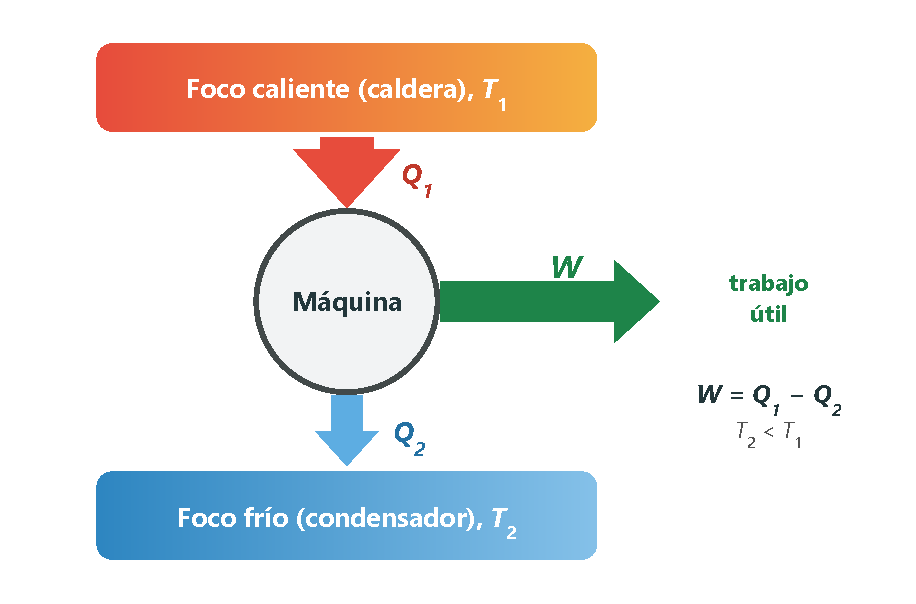
\includegraphics[width=0.6\textwidth]{images/UD13/maquina_termica}
    \caption{Esquema de una máquina térmica.}
    \label{fig:ud13-maquina}
\end{figure}

El \textbf{rendimiento} es la fracción del calor absorbido que se convierte en trabajo:
\[ \eta = \frac{|W|}{|Q_1|} = \frac{|Q_1| - |Q_2|}{|Q_1|} \]
Una consecuencia del segundo principio es que siempre \(\eta < 1\): \textbf{no es posible transformar íntegramente en trabajo el
calor absorbido} (enunciado de Kelvin-Planck). Carnot demostró que ninguna máquina que trabaje entre dos focos puede superar el
rendimiento de una máquina ideal reversible, la \textbf{máquina de Carnot}:
\[ \eta_{\text{máx}} = 1 - \frac{T_2}{T_1} \qquad \text{(temperaturas en kelvin)} \]

Son máquinas térmicas la máquina de vapor, las turbinas de las centrales térmicas y los \textbf{motores de combustión}, como el
motor de cuatro tiempos de los coches (figura~\ref{fig:ud13-motor}). Los \textbf{frigoríficos} y las \textbf{bombas de calor} son
máquinas térmicas que funcionan al revés: con un trabajo, extraen calor de un foco frío y lo ceden a uno caliente.

\begin{figure}[H]
    \centering
    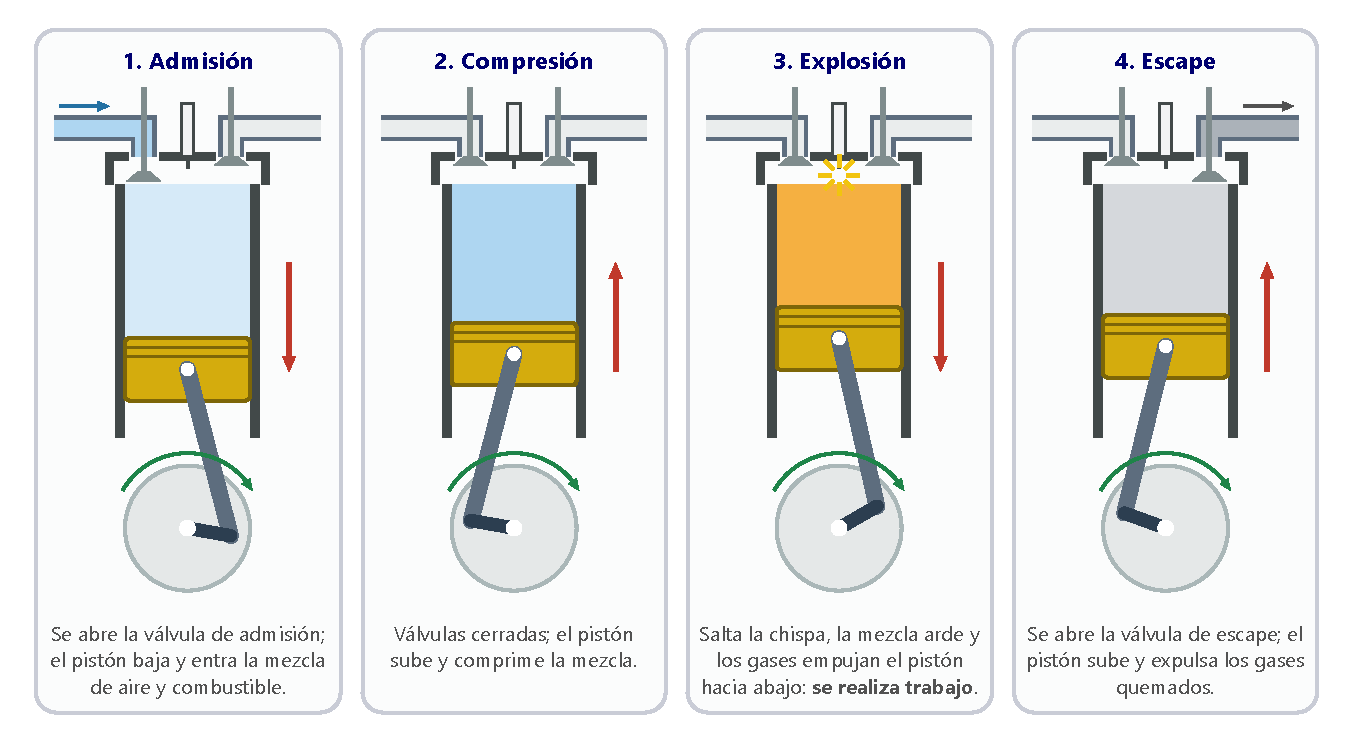
\includegraphics[width=\textwidth]{images/UD13/motor_cuatro_tiempos}
    \caption{Los cuatro tiempos de un motor de gasolina.}
    \label{fig:ud13-motor}
\end{figure}

\begin{example}
    \textbf{Rendimiento de un motor.} Un motor térmico realiza un trabajo de \qty{160}{\joule} en cada ciclo, y absorbe
    \qty{130}{\calorie} del foco caliente. a) Calcula su rendimiento. b) ¿Qué calor cede al foco frío en cada ciclo? c) Si trabaja
    entre \qty{500}{\degreeCelsius} y \qty{30}{\degreeCelsius}, ¿cuál sería su rendimiento máximo?

    \textbf{Solución.} a) \(Q_1 = 130 \cdot \num{4.18} = \qty{543.4}{\joule}\);
    \(\eta = \dfrac{160}{\num{543.4}} = \num{0.294}\), es decir, un \qty{29.4}{\percent}.

    b) \(|Q_2| = |Q_1| - |W| = \num{543.4} - 160 = \qty{383}{\joule}\).

    c) \(\eta_{\text{máx}} = 1 - \dfrac{303}{773} = \num{0.608}\), un \qty{60.8}{\percent}. El motor real queda lejos del ideal por
    el rozamiento, las pérdidas de calor y la irreversibilidad de la combustión.
\end{example}

\begin{exercise}
    Indica razonadamente si aumenta o disminuye la entropía del sistema en cada caso: a) se funde un cubito de hielo; b) ordenas tu
    cuarto; c) calientas una barra de hierro; d) congelas un caldo; e) preparas un café con leche; f) arde una hoguera.
    \begin{solu}
        Aumenta en \textcolor{red}{a, c, e y f} (más desorden: fusión, mayor agitación, mezcla, formación de gases). Disminuye en
        \textcolor{red}{b y d} (más orden); en b, la entropía del universo aumenta igualmente por el calor que desprende nuestro
        cuerpo al trabajar.
    \end{solu}
\end{exercise}

\begin{exercise}
    Pronostica cómo cambia la entropía en estas reacciones: a) \ch{2 H2O2(aq) -> 2 H2O(l) + O2(g)}; b) \ch{N2(g) + 3 H2(g) -> 2
    NH3(g)}; c) \ch{CaCO3(s) -> CaO(s) + CO2(g)}; d) \ch{H2O(g) -> H2O(l)}.
    \begin{solu}
        a) \textcolor{red}{Aumenta} (se forma un gas). b) \textcolor{red}{Disminuye} (de 4 a 2 moles de gas). c)
        \textcolor{red}{Aumenta} (se forma un gas a partir de un sólido). d) \textcolor{red}{Disminuye} (condensación).
    \end{solu}
\end{exercise}

\begin{exercise}
    Una máquina térmica absorbe \qty{2000}{\joule} del foco caliente y cede \qty{1400}{\joule} al foco frío en cada ciclo. Calcula el
    trabajo que realiza y su rendimiento.
    \begin{solu}
        \(|W| = 2000 - 1400 = \textcolor{red}{\qty{600}{\joule}}\); \(\eta = \dfrac{600}{2000} = \textcolor{red}{\qty{30}{\percent}}\).
    \end{solu}
\end{exercise}

%========================================================================================
\section{Física en la vida: energía solar fotovoltaica y termodinámica}\label{sec:ud13-solar}
%========================================================================================

España recibe entre \num{2500} y \num{3000} horas de sol al año, así que la \textbf{energía solar} es una alternativa limpia y
rentable a los combustibles fósiles. Hay dos formas principales de aprovecharla en una vivienda.

Los \textbf{paneles fotovoltaicos} transforman directamente la luz en electricidad. Están formados por células de silicio, un
semiconductor que absorbe los fotones y libera electrones, lo que produce una corriente continua; un \textbf{inversor} la convierte
en alterna para usarla en casa. Necesitan un mínimo de radiación solar para funcionar y duran entre 25 y 30 años.

Los \textbf{paneles solares térmicos} calientan un líquido que circula por su interior y se usan para la calefacción y el agua
caliente sanitaria (ACS). Una variante son los \textbf{paneles solares termodinámicos}: en realidad son una \textbf{bomba de calor}.
Por ellos circula un líquido refrigerante que hierve a muy baja temperatura y se evapora absorbiendo calor del ambiente, incluso de
noche, con lluvia o a temperaturas por debajo de cero. Un compresor aumenta la presión del gas, y con ella su temperatura; después
el gas se condensa en un intercambiador y cede su calor al agua de un depósito aislado. Como en un frigorífico, con un pequeño
trabajo eléctrico se traslada calor de un foco frío (el aire exterior) a uno caliente (el agua): cada kilovatio hora eléctrico puede
llevar al agua tres o cuatro kilovatios hora de calor. También se investiga en \textbf{paneles híbridos}, que generan a la vez
electricidad y agua caliente; además, al refrigerar las células, mejoran su rendimiento eléctrico.

\begin{exercise}
    a) ¿Qué transformaciones de energía tienen lugar en un panel fotovoltaico y en un panel termodinámico? b) Un panel termodinámico
    entrega \qty{3.5}{\kilo\watt\hour} de calor al agua por cada \qty{1}{\kilo\watt\hour} eléctrico que consume el compresor. ¿Viola
    esto el primer principio? ¿De dónde sale el resto de la energía? c) Investigad qué es la energía \textbf{agrovoltaica} y por qué
    interesa en el sector agrícola.
    \begin{solu}
        a) Fotovoltaico: \textcolor{red}{radiante \(\rightarrow\) eléctrica}. Termodinámico: \textcolor{red}{eléctrica \(\rightarrow\)
        trabajo del compresor}, y el calor del ambiente pasa al agua. b) \textcolor{red}{No}: los \qty{2.5}{\kilo\watt\hour}
        restantes son \textcolor{red}{calor extraído del aire exterior}; el compresor solo lo «bombea» del foco frío al caliente.
        c) \textcolor{red}{Respuesta abierta} (placas solares sobre cultivos o pastos: se comparte el terreno, se da sombra y se
        reduce la evaporación del agua).
    \end{solu}
\end{exercise}

%========================================================================================
\section{Prácticas}\label{sec:ud13-practicas}
%========================================================================================

\subsection{Una nube en una botella}

\noindent\begin{minipage}[t]{0.48\textwidth}
    \textbf{Objetivo}
    \begin{itemize}
        \item Comprobar que una expansión casi adiabática enfría un gas y relacionarlo con el primer principio y con la formación de
        las nubes.
    \end{itemize}
\end{minipage}\hfill
\begin{minipage}[t]{0.48\textwidth}
    \textbf{Material}
    \begin{itemize}
        \item Una botella de plástico de \qty{2}{\litre} con tapón, un poco de agua tibia, una cerilla (o alcohol de farmacia) y,
        si se dispone de ella, una bomba de bicicleta con un tapón perforado y una válvula.
    \end{itemize}
\end{minipage}

\begin{figure}[H]
    \centering
    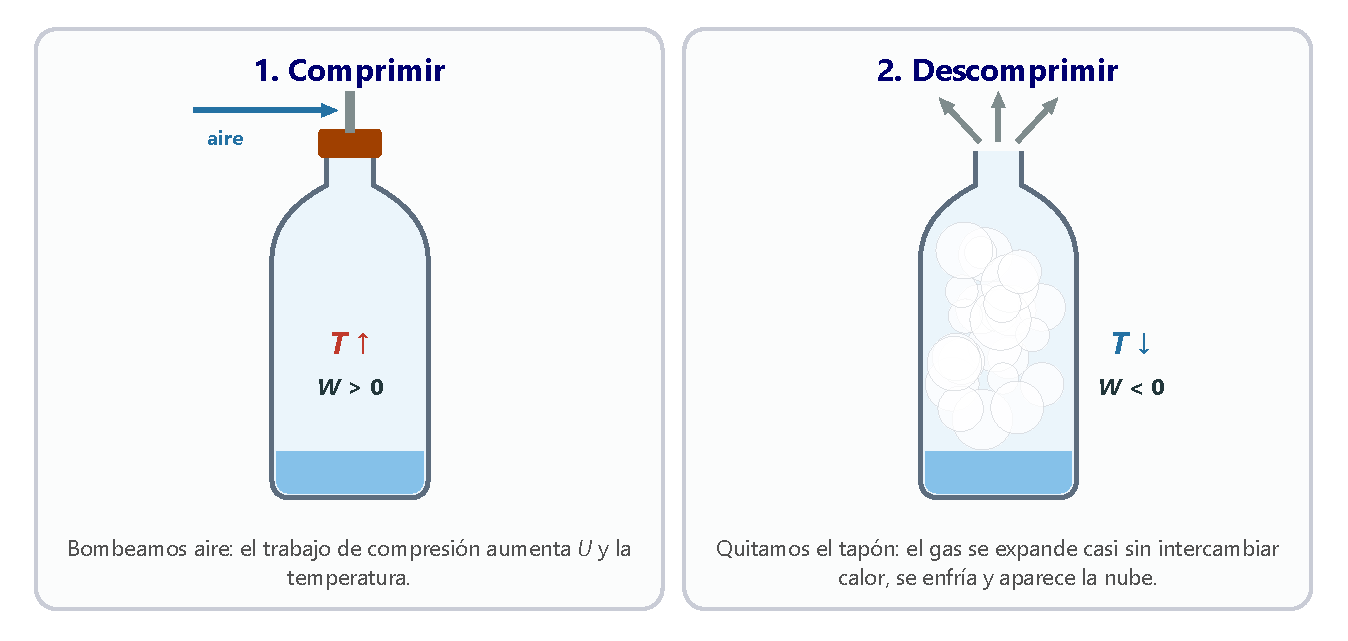
\includegraphics[width=0.75\textwidth]{images/UD13/practica_nube}
    \caption{Al descomprimir el aire de la botella, se enfría y se forma una nube.}
    \label{fig:ud13-nube}
\end{figure}

\textbf{Procedimiento}
\begin{enumerate}[label=\numberballgreen]
    \item Echa un dedo de agua tibia en la botella y agítala para que el aire se cargue de vapor. Vacía el agua.
    \item Enciende una cerilla, apágala y mete el humo en la botella (las partículas de humo sirven de núcleos de condensación,
    como el polvo en la atmósfera). Tapa la botella. Con la supervisión del profesor, se puede usar en su lugar unas gotas de alcohol.
    \item Comprime el aire: aprieta la botella con fuerza unos segundos, o bombea aire con la bomba de bicicleta.
    \item Suelta la botella de golpe (o quita el tapón): en el interior aparece una nube. Si vuelves a apretar, desaparece.
\end{enumerate}

\begin{exercise}
    a) Aplica el primer principio a la compresión y a la expansión del aire de la botella. ¿Por qué podemos considerar que los
    procesos son adiabáticos? b) ¿Por qué aparece la nube? c) Relaciona la experiencia con la formación de las nubes al ascender el
    aire en la atmósfera.
    \begin{solu}
        a) Son tan rápidos que \textcolor{red}{no da tiempo a intercambiar calor}: \(Q \approx 0\) y \(\Delta U = W\). Al
        comprimir, \(W > 0\): \(U\) y la temperatura aumentan. Al expandirse, \(W < 0\): \textcolor{red}{\(U\) y la temperatura
        disminuyen}. b) Al enfriarse, el aire no puede contener tanto vapor y este \textcolor{red}{se condensa} en gotitas sobre las
        partículas de humo. c) El aire que asciende encuentra \textcolor{red}{menor presión, se expande casi adiabáticamente y se
        enfría} (unos \qty{10}{\degreeCelsius} por kilómetro si está seco: es el gradiente adiabático); al llegar al punto de rocío, el
        vapor se condensa y se forma la nube.
    \end{solu}
\end{exercise}

\subsection{Calor específico de un metal}

\noindent\begin{minipage}[t]{0.48\textwidth}
    \textbf{Objetivo}
    \begin{itemize}
        \item Determinar el calor específico de un metal mediante un calorímetro e identificar el metal.
    \end{itemize}
\end{minipage}\hfill
\begin{minipage}[t]{0.48\textwidth}
    \textbf{Material}
    \begin{itemize}
        \item Un calorímetro (o un vaso de poliestireno con tapa), un termómetro, una balanza, un vaso de precipitados, un hornillo, hilo y una
        pieza metálica de unos \qty{150}{\g}.
    \end{itemize}
\end{minipage}

\begin{figure}[H]
    \centering
    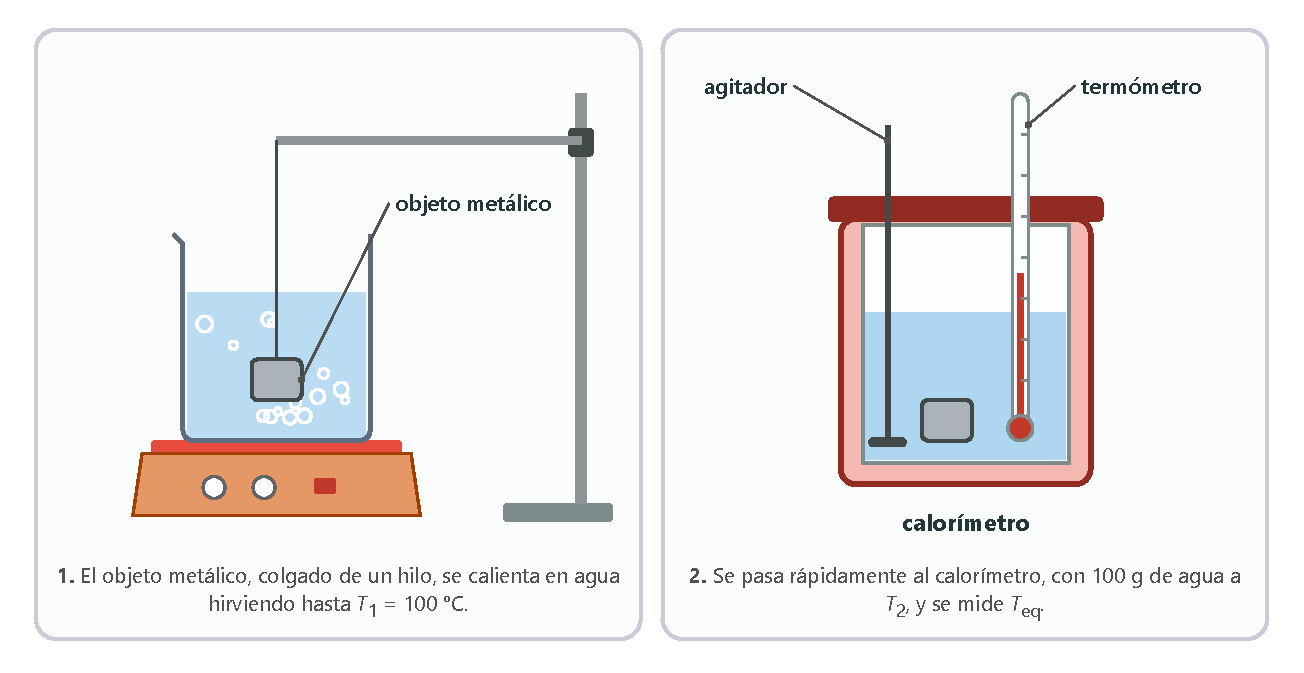
\includegraphics[width=0.75\textwidth]{images/UD13/practica_calor_especifico}
    \caption{Medida del calor específico de un metal.}
    \label{fig:ud13-practica-ce}
\end{figure}

\textbf{Procedimiento}
\begin{enumerate}[label=\numberballgreen]
    \item Pesa la pieza metálica (\(m_1\)), átala con un hilo y sumérgela en agua hirviendo varios minutos: su temperatura será
    \(T_1 = \qty{100}{\degreeCelsius}\).
    \item Echa en el calorímetro una masa conocida de agua (\(m_2\), por ejemplo \qty{200}{\g}) y mide su temperatura, \(T_2\).
    \item Pasa rápidamente la pieza al calorímetro, tápalo, agita y anota la temperatura máxima que alcanza: es \(T_{eq}\).
    \item Con el balance \(m_1\,c_1\,(T_{eq} - T_1) + m_2\,c_{\text{agua}}\,(T_{eq} - T_2) = 0\), calcula \(c_1\) y compáralo con la
    tabla~\ref{tab:ud13-calor-especifico}.
\end{enumerate}

\begin{exercise}
    En la práctica, una pieza de \qty{150}{\g} a \qty{100}{\degreeCelsius} se introduce en \qty{200}{\g} de agua a \qty{20}{\degreeCelsius},
    y el equilibrio se alcanza a \qty{25.2}{\degreeCelsius}. a) Calcula el calor específico del metal. ¿De qué metal se trata? b) ¿El
    valor obtenido será algo mayor o algo menor que el real si el calorímetro pierde calor? ¿Por qué?
    \begin{solu}
        a) \(c_1 = \dfrac{m_2\,c_{\text{agua}}\,(T_{eq} - T_2)}{m_1\,(T_1 - T_{eq})} = \dfrac{\num{0.2} \cdot 4180 \cdot \num{5.2}}{\num{0.15}
        \cdot \num{74.8}} = \textcolor{red}{\qty{387}{\joule\per\kg\per\kelvin}}\): es \textcolor{red}{cobre}. b)
        \textcolor{red}{Menor}: parte del calor del metal se pierde, el agua se calienta menos de lo que debería y parece que el metal
        cedió menos energía.
    \end{solu}
\end{exercise}

%========================================================================================
\section{Situación de aprendizaje: el deshielo del Ártico (ODS 13 y 14)}\label{sec:ud13-ods}
%========================================================================================

El \textbf{ODS 13} pide adoptar medidas urgentes para combatir el cambio climático, y el \textbf{ODS 14}, conservar los océanos y los
mares. Ambos están relacionados con el calor. En el último siglo, el aumento del efecto invernadero ha elevado la temperatura media
del planeta más de \qty{1}{\degreeCelsius}, y el Ártico se calienta unas tres o cuatro veces más deprisa que el resto del mundo: desde
1979 ha perdido en torno a un tercio de su hielo marino en verano. Una de las causas es la \textbf{amplificación ártica}: el hielo y
la nieve reflejan la mayor parte de la luz solar, pero el agua del mar, más oscura, la absorbe; al fundirse el hielo, el océano
absorbe más radiación, se calienta y funde todavía más hielo.

Las consecuencias no son solo ambientales (subida del nivel del mar, pérdida de hábitats de especies como el oso polar o la
morsa), también económicas y geopolíticas: por ejemplo, se abren nuevas rutas marítimas por el Ártico. Se estima que cada
tonelada de \ch{CO2} emitida provoca la desaparición de unos \qty{3}{\m\squared} de hielo ártico en verano. Por eso es importante
conocer nuestra \textbf{huella de carbono}, la cantidad de gases de efecto invernadero que emitimos con nuestras actividades.

\begin{marker}
    \textbf{Reto:} por grupos, investigad la relación entre el calor, el deshielo y nuestra huella de carbono, y grabad un podcast
    de un máximo de tres minutos para la radio escolar.
\end{marker}

\begin{enumerate}[label=\numberballred]
    \item \textbf{Investigad} cuánto calor hace falta para fundir el hielo (ejercicio siguiente) y por qué el agua del mar
    tarda tanto en enfriarse y en calentarse (su calor específico).
    \item \textbf{Calculad} vuestra huella de carbono con una calculadora en línea (por ejemplo, la del Ministerio para la
    Transición Ecológica) y comparadla con la media española.
    \item \textbf{Proponed} medidas para reducirla a nivel individual y en el centro: transporte, alimentación, calefacción y
    aire acondicionado, consumo eléctrico.
    \item \textbf{Comunicad}: escribid un guion argumentado y grabad el podcast (con Audacity o una aplicación gratuita del móvil).
\end{enumerate}

\begin{exercise}
    a) ¿Qué energía hace falta para fundir \qty{1}{\tonne} de hielo a \qty{0}{\degreeCelsius}? b) ¿Y para fundir un bloque de hielo
    marino de \qty{3}{\m\squared} de superficie y \qty{1.5}{\m} de espesor? Densidad del hielo: \qty{917}{\kg\per\m\cubed}.
    c) ¿Durante cuánto tiempo tendría que funcionar un radiador de \qty{2}{\kilo\watt} para suministrar esa energía?
    \begin{solu}
        a) \(Q = m\,L_f = 1000 \cdot \num{3.34e5} = \textcolor{red}{\qty{3.34e8}{\joule}}\). b) \(m = 917 \cdot 3 \cdot \num{1.5} =
        \qty{4127}{\kg}\); \(Q = \textcolor{red}{\qty{1.38e9}{\joule}}\). c) \(t = \dfrac{\num{1.38e9}}{2000} = \qty{6.9e5}{\s}
        \approx \textcolor{red}{8 días}\).
    \end{solu}
\end{exercise}
